% Setup - do not change
\documentclass[11pt]{article}
\usepackage[top=0.9in, left=0.9in, bottom=0.9in, right=0.9in]{geometry} 
\usepackage{parskip}
\usepackage{multicol}
\usepackage[english]{babel}
\usepackage[utf8]{inputenc}
\usepackage{amsmath,amsthm,amssymb,graphicx,pdfpages,lipsum,hyperref}
\usepackage[none]{hyphenat}
\usepackage{csquotes}
\usepackage{float}


\setlength\parindent{0pt}
%%%%%%%%%%%%%%%%%%%%%%%%%%%%%%%%%%%%%%%%%%%%%%%%%%%%%%%%%%%%%%%%%%%
% add other packages here if required

%% Bibliography are specified in this file. You can also choose inline bib style if you want to. But make sure your citation style is consistent (and proper)
% For more details on citation: https://library.unimelb.edu.au/recite
\usepackage[sorting = none]{biblatex}
\addbibresource{references.bib}

%%%%%%%%%%%%%%%%%%%%%%%%%%%%%%%%%%%%%%%%%%%%%%%%%%%%%%%%%%%%%%%%%%% the '%' symbol denotes comments

% Begin document creation
% DELETE THE \lipsum PLACEHOLDERS WHEN YOU BEGIN
\title{\textbf{How Does Viral Infection Affect Taxi Service Reliance?} \\ 
MAST30034 Assignment 1}
\author{
Xavier Travers \\
Student ID: 1178369 \\
%% Replace the link with your github repo
% 1. Remember to escape underscore in the link.
% 2. Remember to include the commit you want to submit in the link
TODO: \href{https://github.com/MAST30034-Applied-Data-Science/mast30034\_p1\_template/tree/fd9f1dd17fdbcb5b119b70c93a22da8210d44fd7}{Github Repository}
}

\begin{document}
\maketitle

\section{Introduction}
% Link to a 30 min tutorial if you require revision: https://www.overleaf.com/learn/latex/Learn_LaTeX_in_30_minutes

Viruses are currently on everyone's due to the COVID-19 pandemic.
With the shift to working from home, lockdowns and fears of infection, 
it is natural to assume that people-facing industries are no longer relied upon to the same degree.
% it is a natural assumption that many people-facing industries such as ride-hailing have suffered in demand.
To what extent is such an assumption true?
This report investigates possible correlations between measures of reliance on taxi services, and virus case rates.
While most research is satisfied with measuring correlations with demand in the form of usage frequency, 
the focus for this report is placed on measurements which reflect reliance more than demand.

Specific to taxi services, two key measurements of reliance are average travel radius/distance and average passenger count.
Both of these measurements will correlate to the level of trust the average person places in a taxi service over its alternatives.
For example, one may trust their own cars for interstate travel, 
but may be happy to pay for a street-hail on the way home from work (and similar logic may apply to trust in taxis with numbers of passengers).

Detailed throughout this report are steps taken to model average weekly trip distances and passenger counts against
the case rates of two key viruses of recent importance: COVID-19 and Influenza.

\subsection{Timeline}
Throughout this report, two timelines are used.
\begin{itemize}
    \item \textbf{Timeline 1:} Starting in July 2018 and ending in June 2021.
    This 36-month timeline is used exclusively for time-series plots.
    % \item \textbf{Timeline 2:} Starting in July 2018 and ending in June 2019.
    % This 12-month timeline provides a window of time prior to the COVID-19 pandemic.
    % It is used when data analysis focuses only on the effects of the Influenza virus 
    % (since the effects of COVID-19 are likely confounding).
    \item \textbf{Timeline 2:} Starting in July 2020 and ending in June 2021.
    This 12-month timeline provides a window of time during the COVID-19 pandemic.
    This timeline is used to construct linear models and generate other all other visualizations.
\end{itemize}
Data from 2022 is not included, as many of the datasets would be incomplete or unchecked.
Data from before 2018 is not included to reduce code runtime when generating visualizations.

\subsection{Datasets}
\begin{itemize}
    \item The New York City Taxi and Limousine Commission (TLC) provides a dataset of taxi service trips which captures information such as type of taxi, travel distance, general pickup/dropoff locations/times and driver-input passenger counts \cite{tlcdataset}. 
In this report, the focus is placed on New York's Yellow street hail taxis. The dataset provides coverage over the whole of Timeline 2.
Also included from the same source is a mapping dataset for the pickup/dropoff location IDs included in the TLC dataset \cite{tlcdataset}.
    \item Influenza case rates are recorded on a weekly basis by the New York Department of Health \cite{fludataset}. 
Case rates in this dataset are dated based on Morbidity and Mortality Weekly Report (MMWR) weeks, which are generated using rules defined by the CDC \cite{mmwr}.
Each entry in this dataset contains an MMWR week, county (within the state of New York), type of Influenza (A, B or unspecified), and case count.
The dataset provides coverage over the whole of Timeline 1.
    \item COVID-19 case rates have been recorded daily by the New York Department of Health and Mental Hygiene \cite{coviddataset}.
This dataset begins on the last day of february, when the first official cases of COVID-19 were recorded in New York City. 
Each entry in this data set contains a date and several of the daily COVID-19 rates by borough (e.g. count of hospitalizations on the day in the Bronx).
Of specific interest is the daily case count per borough.
    \item Since data is aggregated by borough, the population of each borough needs to be accounted for.
    For this purpose, the United States Census Bureau's yearly county population totals data is used \cite{populations2019, populations2020}.
    This report specifically relies on the population estimates for the counties of New York State.
    \item To provide a homogeneous time metric for aggregation, a dataset is generated which defined the MMWR weeks of the data within the selected timeline.
    The MMWR weeks are generated according to the CDC's defined business rules \cite{mmwr}.
    \item For geospatial visualizations, 
    the City of New York's Department of City Planning provides a dataset containing borough outlines \cite{boroughdataset}.
    This contains the geometry of each borough as well as their names.
\end{itemize}


% \LaTeX{} Have many caveats, you should search stack overflow for latex tips whenever you feel something looks bad, for instance:
% When `` quoting '', should be used instead of ". For example, ``test'' vs "test".

% % use \textbf{} for bold text and \textit{} for italic. 
% % \texttt{} creates code blocks akin to `code ticks` in markdown
% \textbf{Please refer to the spec, the word count and page count is strict.} Feel free to change the section headings (and we recommend you do).

% Always remember to cite materials that does not belong to you. For instance, you should cite the sensor datasets \cite{2022sensorreading, 2022sensorlocation}.
% % Example here used biblatex to manage citations: https://www.overleaf.com/learn/latex/Bibliography_management_with_biblatex , You are free to choose your own way for managing references if biblatex seems too hard.

% \lipsum[7]

% You can have \section{}, \subsection{}, and \subsubsection{}
\section{Method}

\subsection{Preprocessing}

The datasets require several preprocessing steps to generate aggregate data for proper analysis.
The flu dataset contains detail only on a weekly basis, 
while the other datasets contain daily data. 
Thus, the most granular time unit by which the data can be analysed is the MMWR week.
While data per day allows for more data-points in analysis,
Timelines 2 and 3 that ensure around 52 aggregated points of data are available for analysis per per borough.

\subsubsection{Cleaning}

There are several processes used to remove outliers and unwanted data.
Noted are the steps taken to ensure that aggregation by borough and MMWR week is achievable with the TLC, COVID-19 and Influenza datasets.
No imputation is necessary, since the scope of the timelines is very wide (approximately 208 million trips' worth), 
and after removing noise (in the methods described below) from the data, there are still approximately 100 million trips.
Neither the COVID-19 nor the Influenza datasets require imputation, 
since these are maintained to the standards of important medical datasets.

\textbf{Borough vs. County:} Each of the 5 boroughs of New York City correspond to a county recognized by New York State \cite{countytoborough}.
Some datasets contain counties, while others define statistics per borough. The boroughs with corresponding counties of different names are: 
Manhattan, which is New York County; 
Staten Island, which is Richmond County;
and Brooklyn, which is Kings County \cite{countytoborough}.

\textbf{Population Dataset:}
Only data for New York City counties within the years of Timeline 1 is kept.

\textbf{TLC Dataset:}
\begin{multicols}{2}
    \begin{enumerate}
        \item Derive trip duration (in hours) and trip speed (in MPH) columns. 
        Filter out illegal (and likely incorrect) trip entries with a speed greater than 65 MPH, 
        as per New York State law \cite{laws}.
        \item Discard all columns except the pickup time, passenger count, trip distance, pickup location ID, and dropoff location ID.
        \item Discard rows with null values in the above columns or where there is negative distance.
        \item Derive the MMWR week associated to each trip entry, as well as the year and month that the majority of the week participates in.
        Discard all rows where the MMWR week is not within Timeline 1.
        \item For each entry, find the associated pickup borough. 
        Discard all rows where either of the location IDs are not within the 5 boroughs.
    \end{enumerate}
\end{multicols}
It is important to note that passenger count is a self-reported metric, 
meaning the original dataset contains many trip records without a recorded passenger count.
Any results from the aggregated data (whether they analyse trip distances or passenger counts) 
only consider the subset of results where a passenger count was defined.
This is not an issue, since after the above cleaning processes,
there are still over 150 million trip records over the span of Timeline 1.

\textbf{COVID-19 and Influenza Datasets:}
This dataset is very simple, and therefore requires very little preprocessing.
First, the case count per day per borough is extracted. 
Then, the MMWR week associated to each entry, as well as the year and month that the majority of the week participates in are derived (where necessary).
Finally, all rows where the MMWR week is not within Timeline 1 are discarded.
For the Influenza dataset, 
counties are converted to their associated borough names for homogeneity of data.

\subsubsection{Aggregation}

\textbf{TLC Dataset:}
This dataset is aggregates by MMWR week and pickup borough.
This allows for a granular look at potential pattern differences between the reliance measures grouped by pickup locations.
The aggregated set is then joined by MMWR year and borough to the corresponding population estimate.
For the groupings described above, the number of trips,
the average trip distance and passenger count is calculated.
This aggregation over Timeline 1 results in approximately $3 \text{ years} \times 12 \text{ months} \times 4 \text{ weeks} = 144 \text{ rows per borough}$.

This report only performs grouping by pickup location,
allowing models to reflect a potential taxi customer's perspective on their immediate surroundings before taking a trip.
However, exploration of differences between grouping by pickup or dropoff location on the results of models 
is a recommended extension to this research.

\textbf{COVID-19 and Influenza Datasets:}
Similarly to the above, the datasets are grouped by MMWR week information and borough where necessary.
This grouping is joined by MMWR year and borough with the corresponding borough's population estimates in a given year.
For each grouping, the weekly case rate per 100'000 people in the borough is calculated.

\textbf{Aggregation Averages:}
Since aggregation is performed on a mass scale, there is the risk of losing a lot of information present in the granularity of per-trip or per-day datasets.
However, aggregating on a mass scale is beneficial in that the averages calculated (for distance and passenger count)
a less prone to variability. As described by the Central Limit Theorem, as sample size $n$ increases for a sample mean $\bar{X}$, 
$\text{var}(\bar{X}) \propto \frac{1}{n}$. Therefore, since there over 150 million trips contained within Timeline 1, the sample size per week per borough is in the hundreds of thousands trips (assuming an even distribution of trips),
minimizing the variance of the sample means used.

\subsection{Analysis and Modelling}

This section of the report highlights the analysis performed on the aggregated data
and describes the models generated for passenger counts and trip distances.

\subsubsection{Preliminary Analysis}

\textbf{Time-Series Analysis:}
It is important to note 
a feature which appears in nearly any time-series that includes 
the months of March to May 2020. 
The following time-series plots will all contain a similar "COVID dip".

Shown in Figure~\ref{fig:ts} is the change in average trip distance over time. Interestingly, 
while most boroughs (pickup or dropoff) experience a slump in average trip distance following the "COVID dip", 
Staten Island appears to recover from the effects, and even increase in average trip distance
during the COVID-19 pandemic.

% \begin{multicols}{2}
    \begin{figure}[H]
        % change the scale multiplier to make the figures smaller or larger
        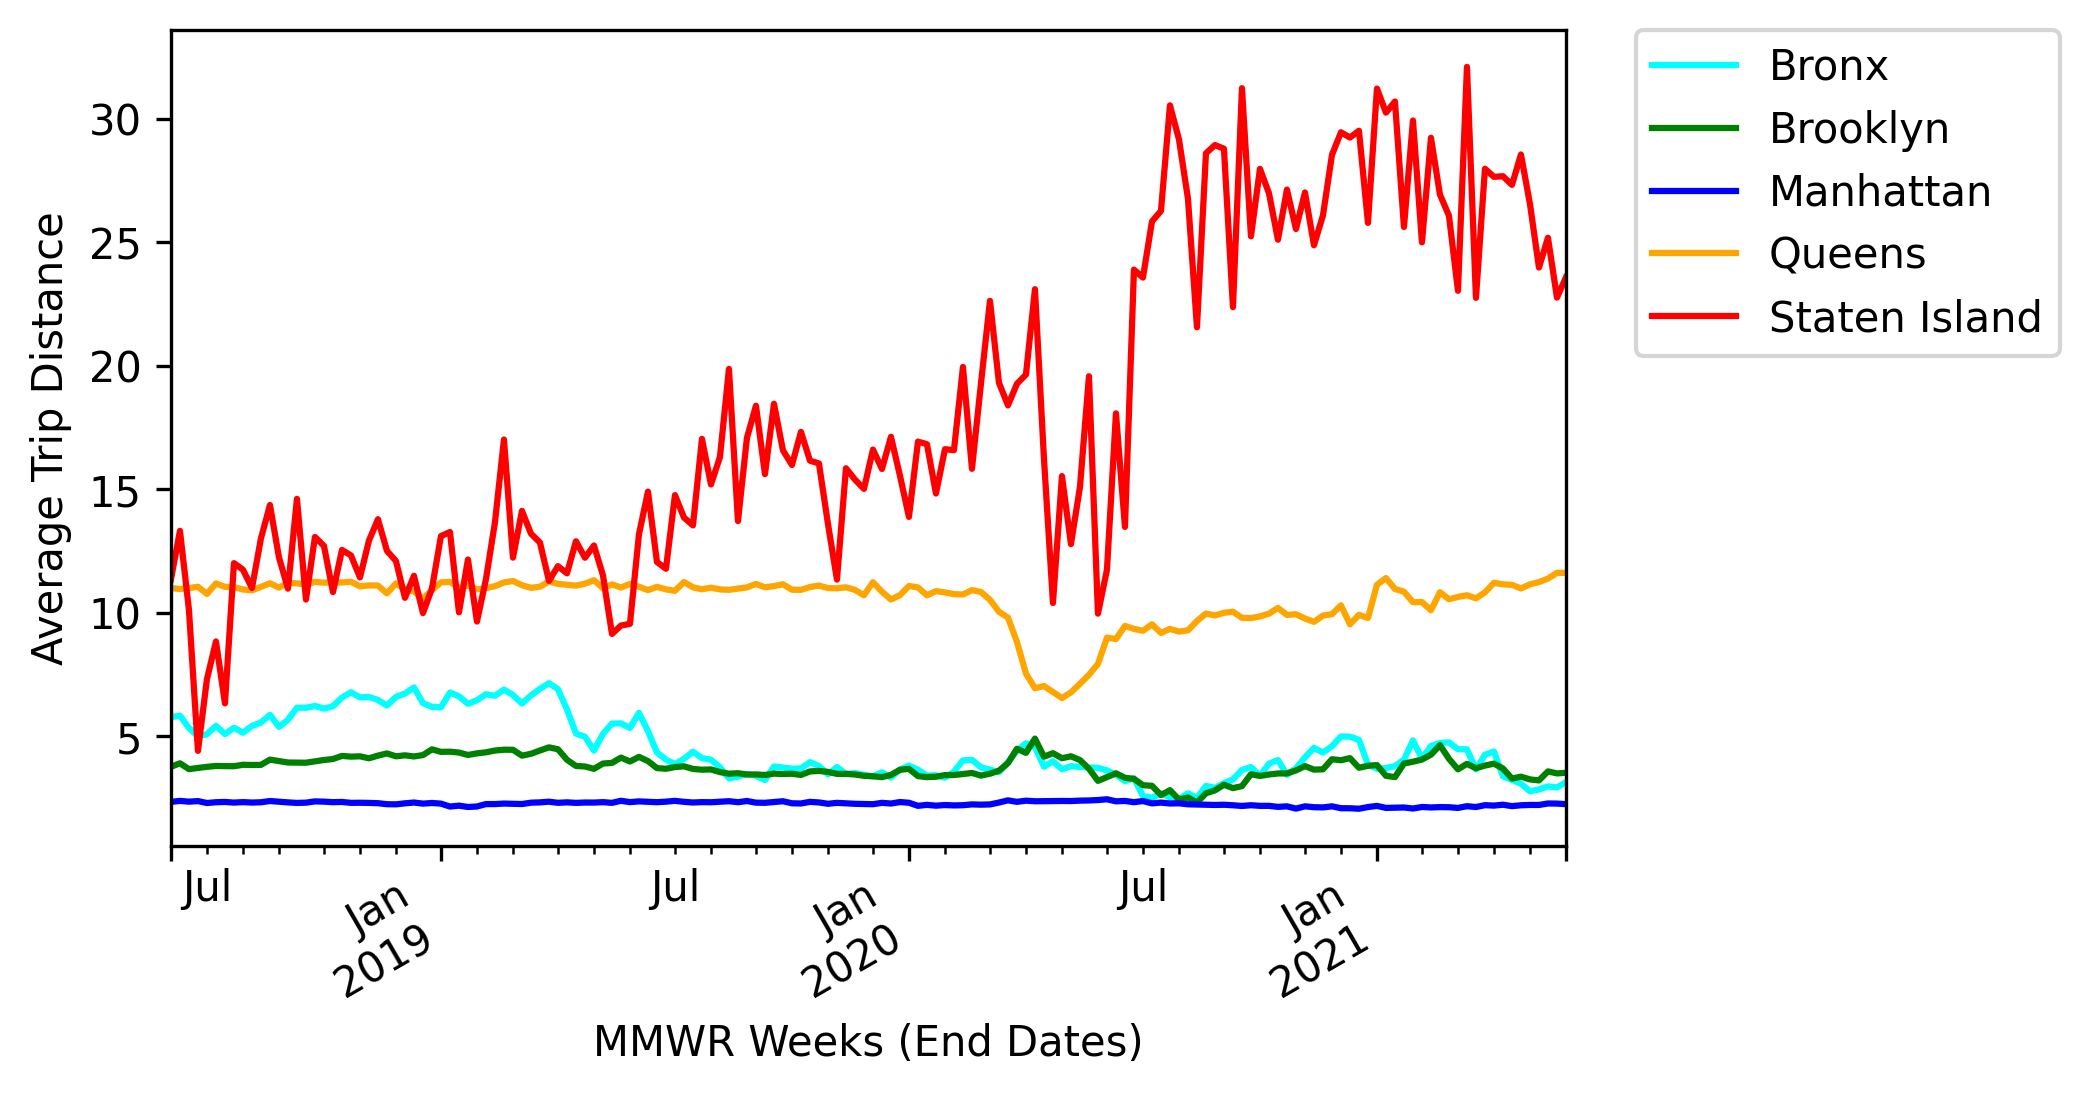
\includegraphics[width=0.5\textwidth]{../plots/time-series-Average Trip Distance-vs-MMWR Weeks (End Dates)-by-pu_borough.png}
        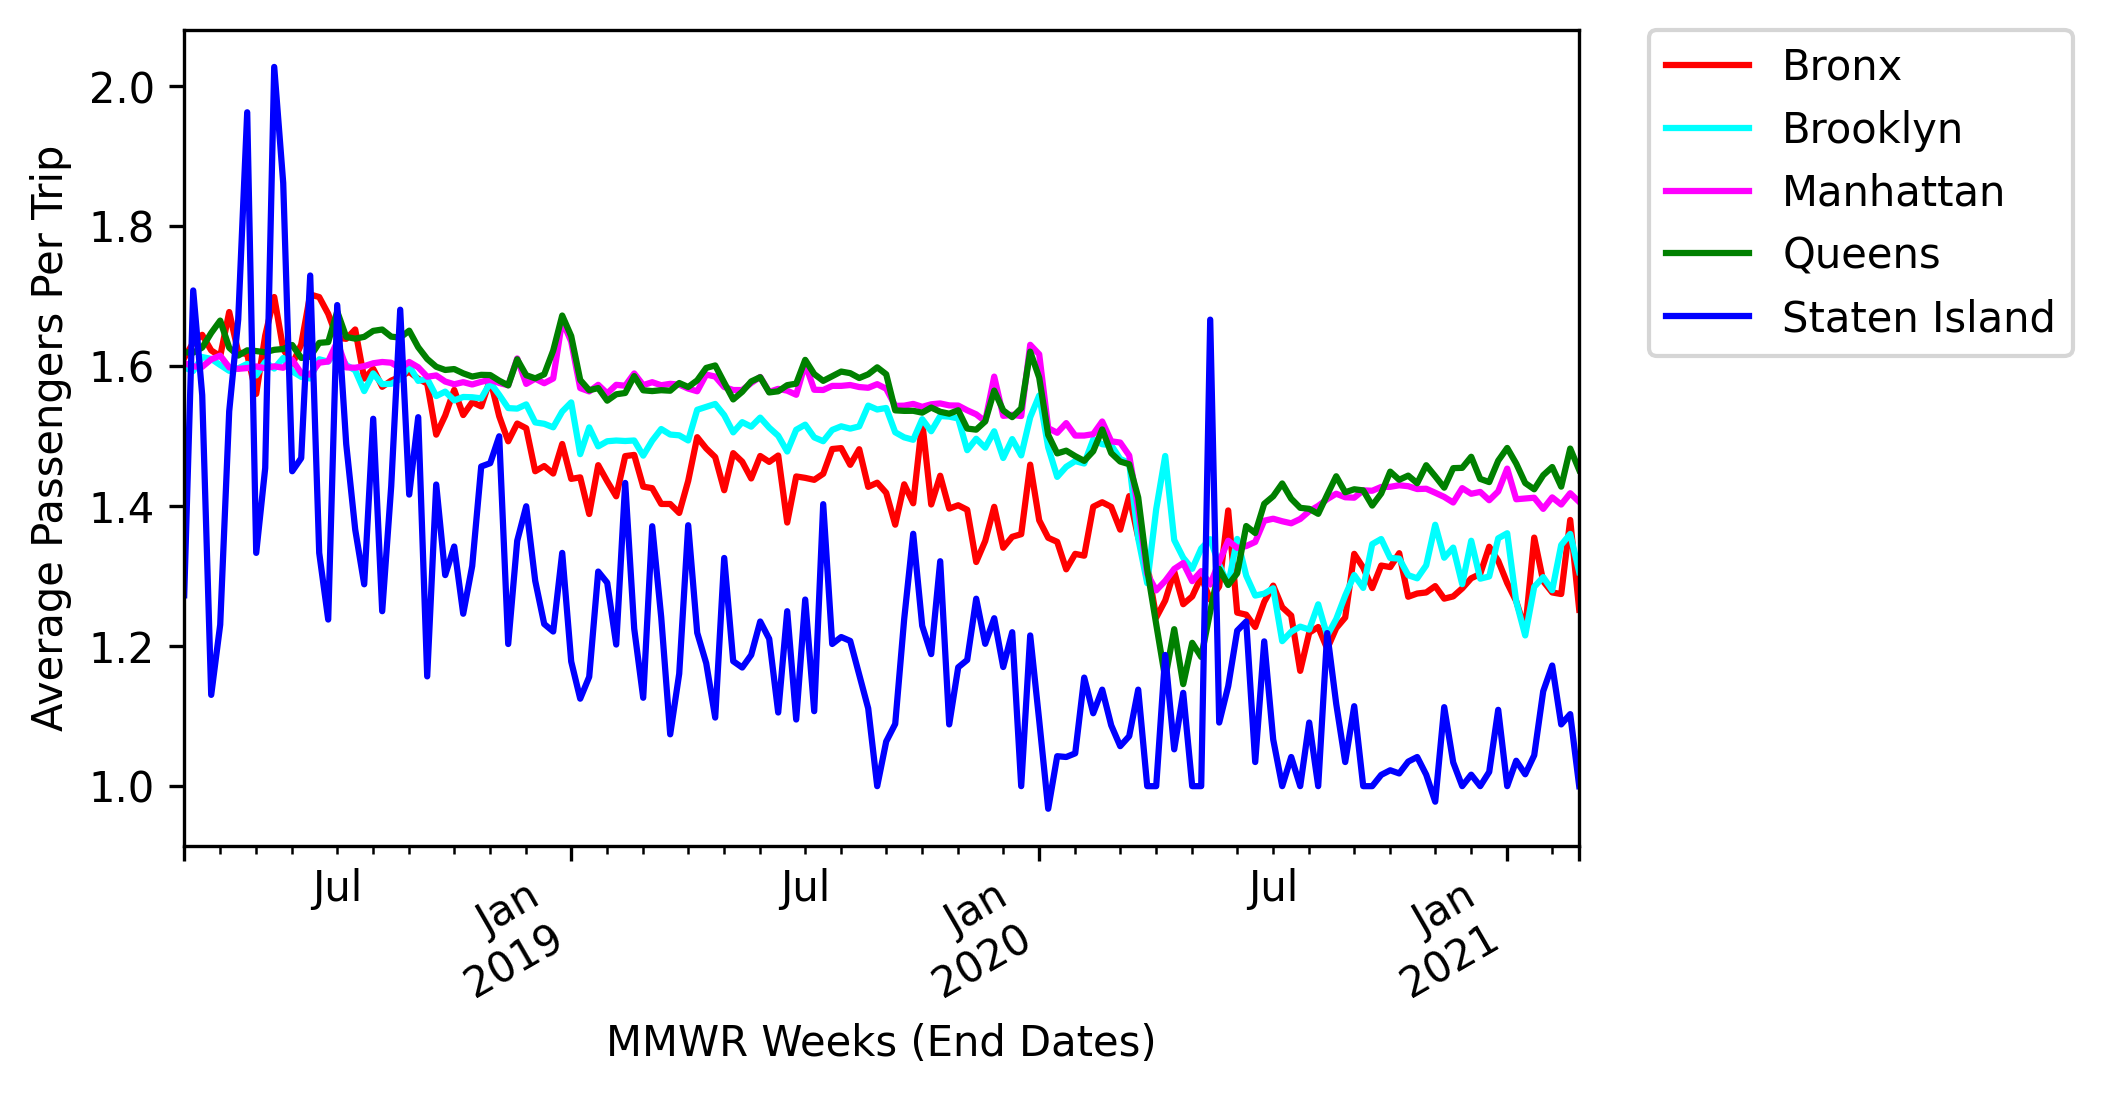
\includegraphics[width=0.5\textwidth]{../plots/time-series-Average Passengers Per Trip-vs-MMWR Weeks (End Dates)-by-pu_borough.png}

        % 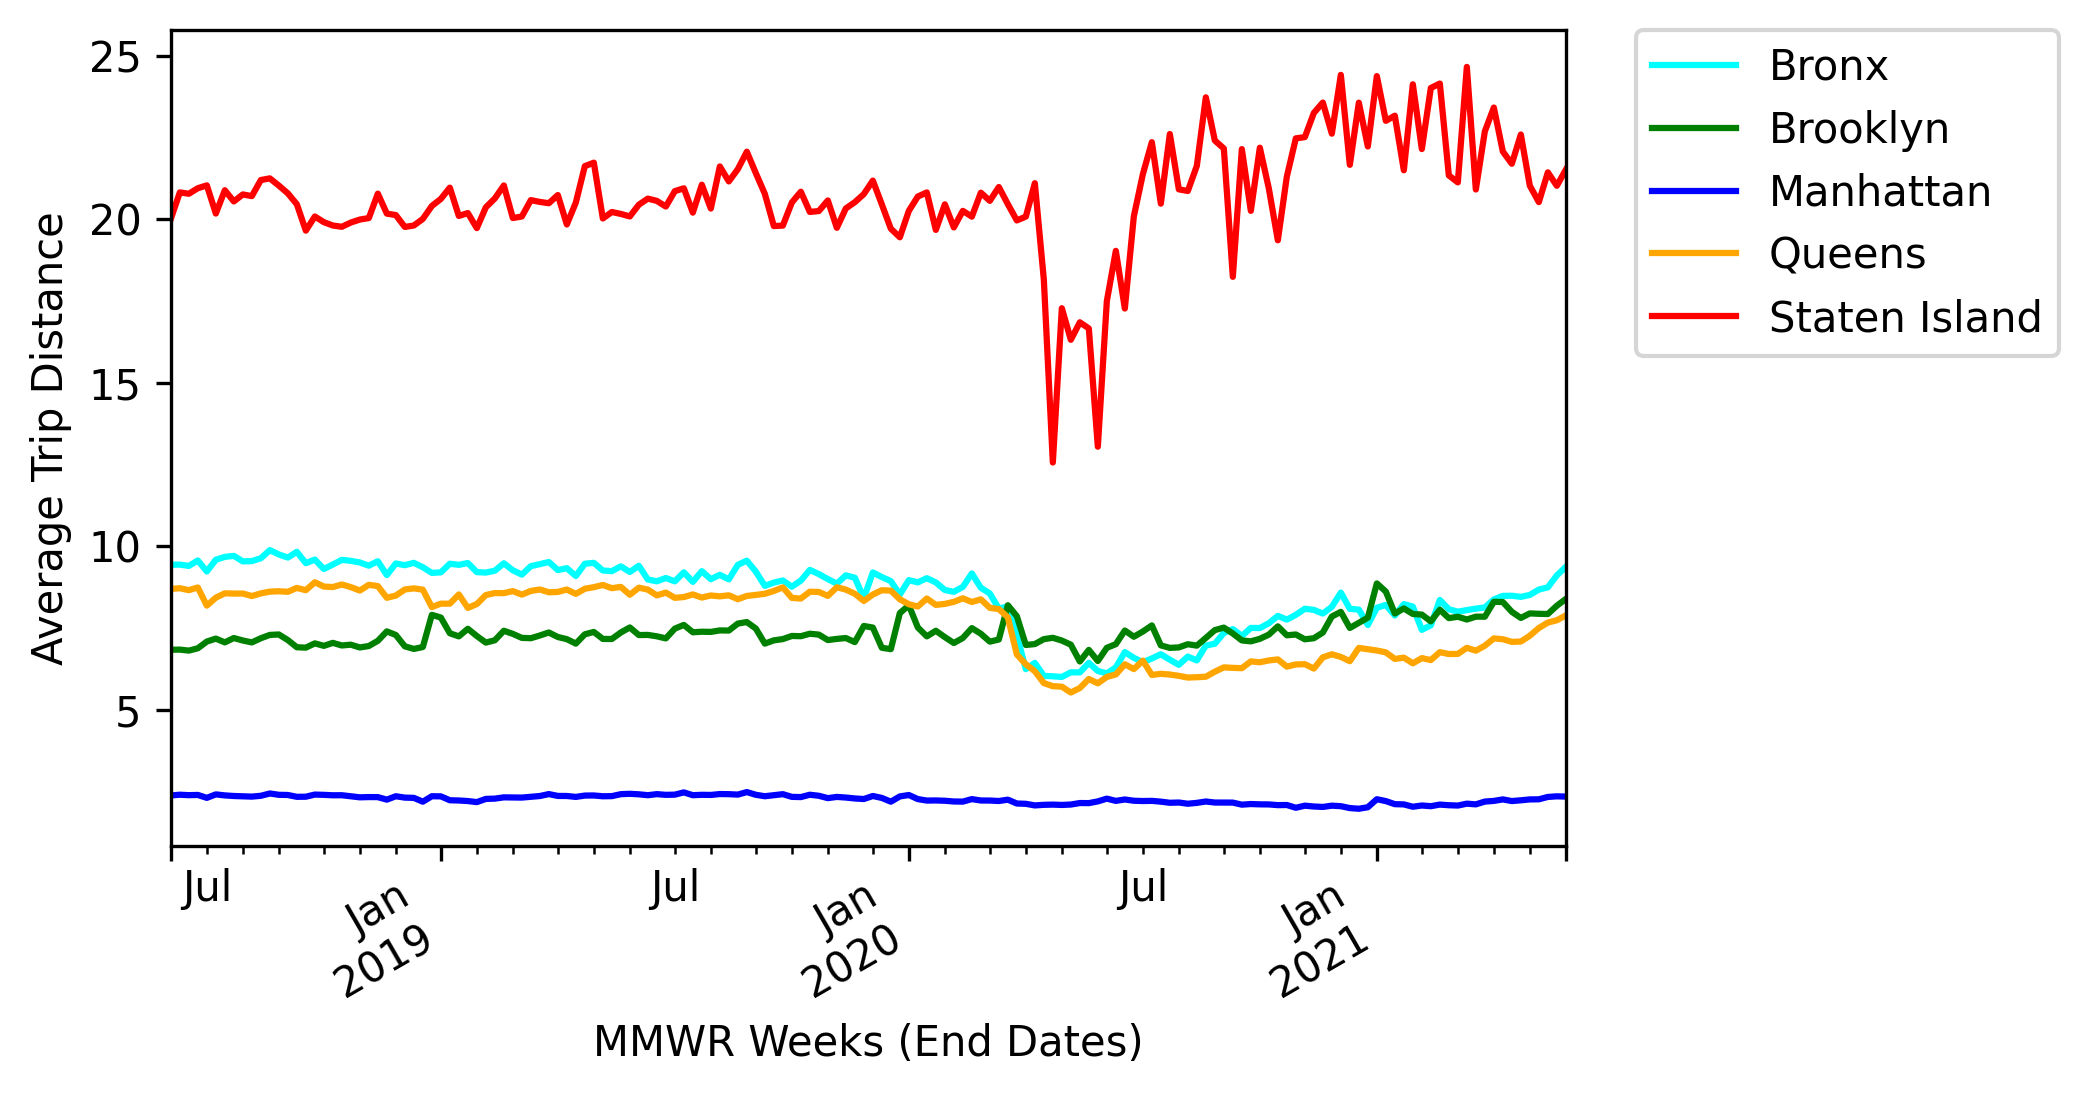
\includegraphics[width=0.45\textwidth]{../plots/time-series-Average Trip Distance-vs-MMWR Weeks (End Dates)-by-do_borough.png}
        % this ensures your figures are centered where possible
        \centering
        \caption{How average trip distances (left) and passenger counts (right) per week per pickup borough vary over time.} % refer to this image as (Figure 1)
        \label{fig:ts}
    \end{figure}

    % \begin{figure}[H]
    %     % change the scale multiplier to make the figures smaller or larger
    %     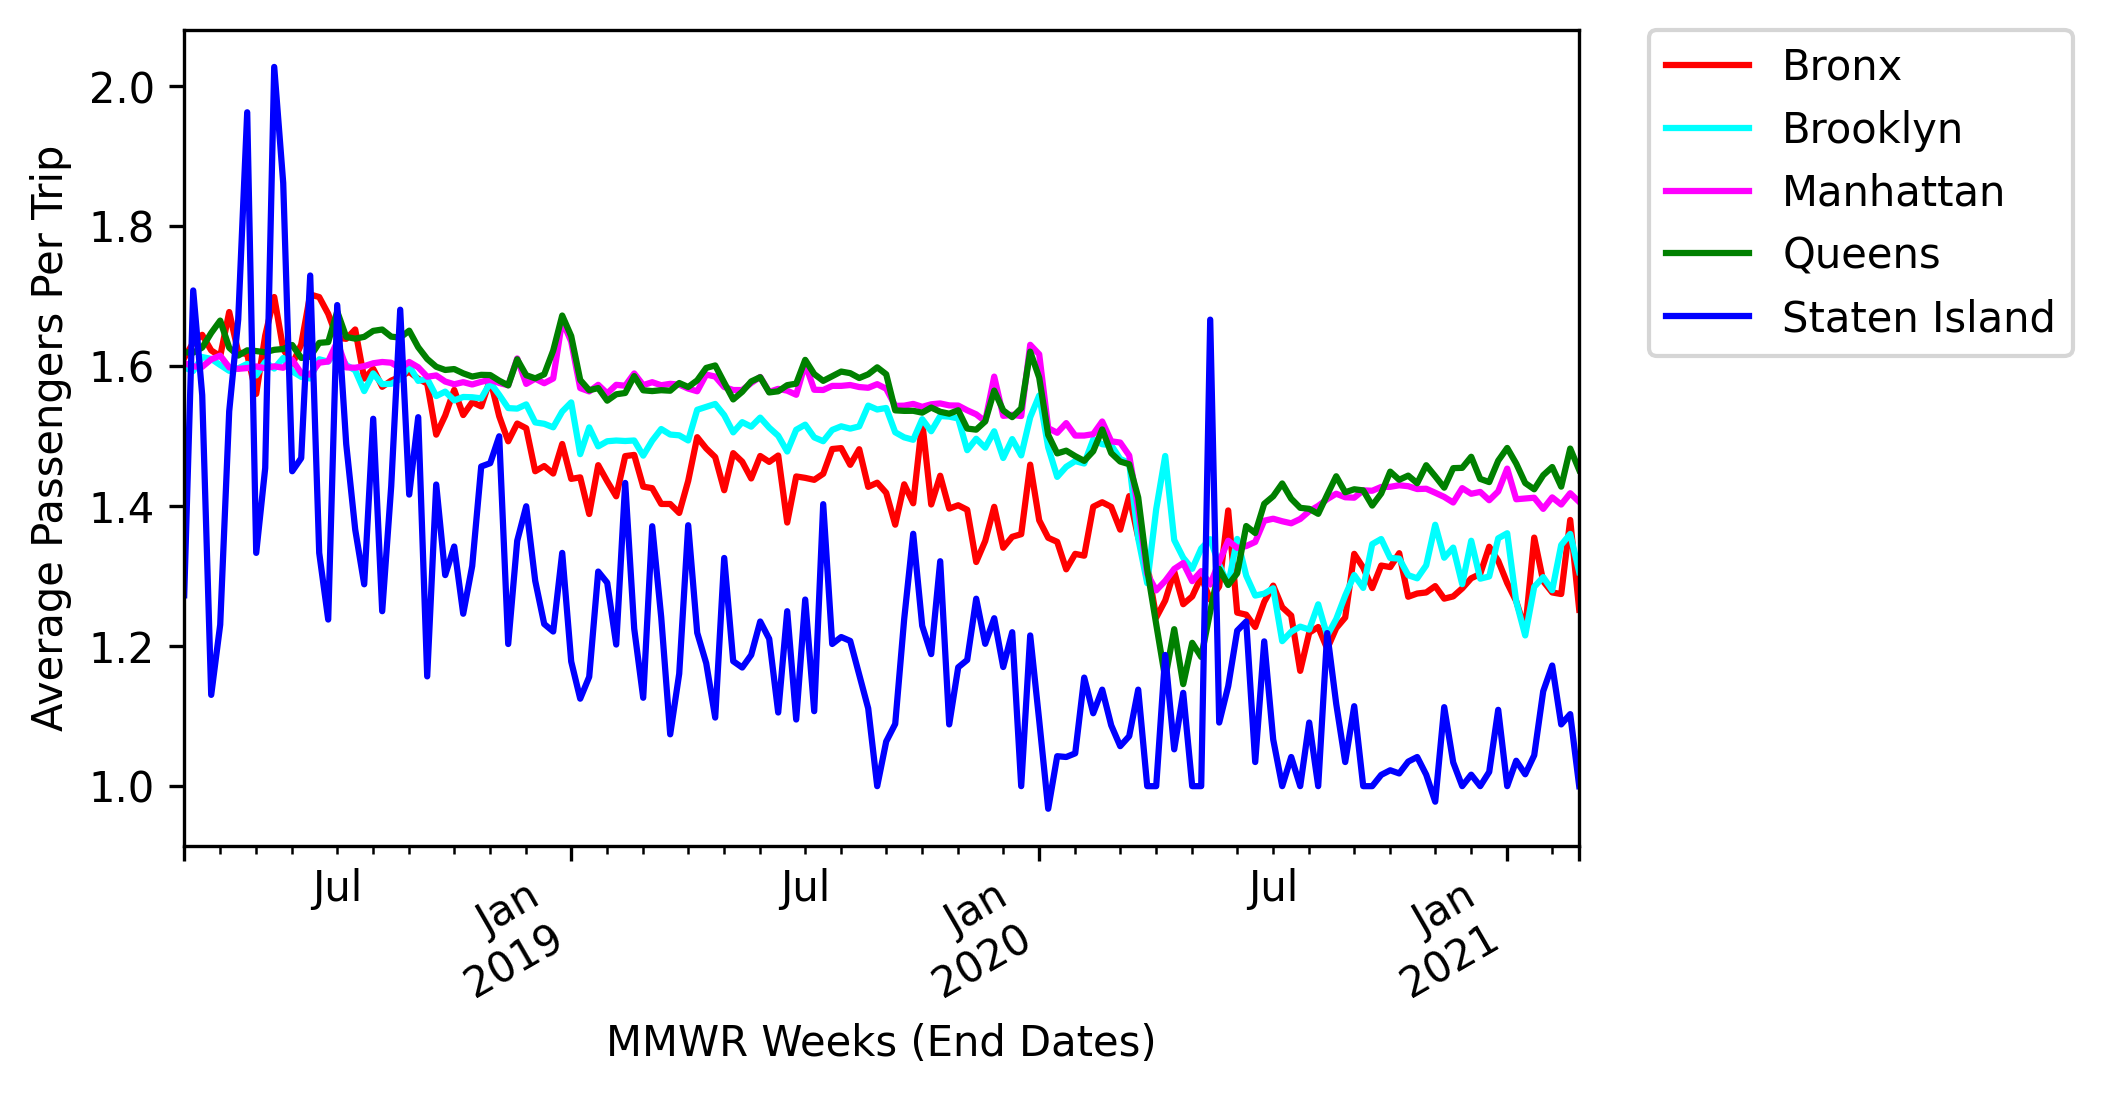
\includegraphics[width=0.5\textwidth]{../plots/time-series-Average Passengers Per Trip-vs-MMWR Weeks (End Dates)-by-pu_borough.png}
    %     % 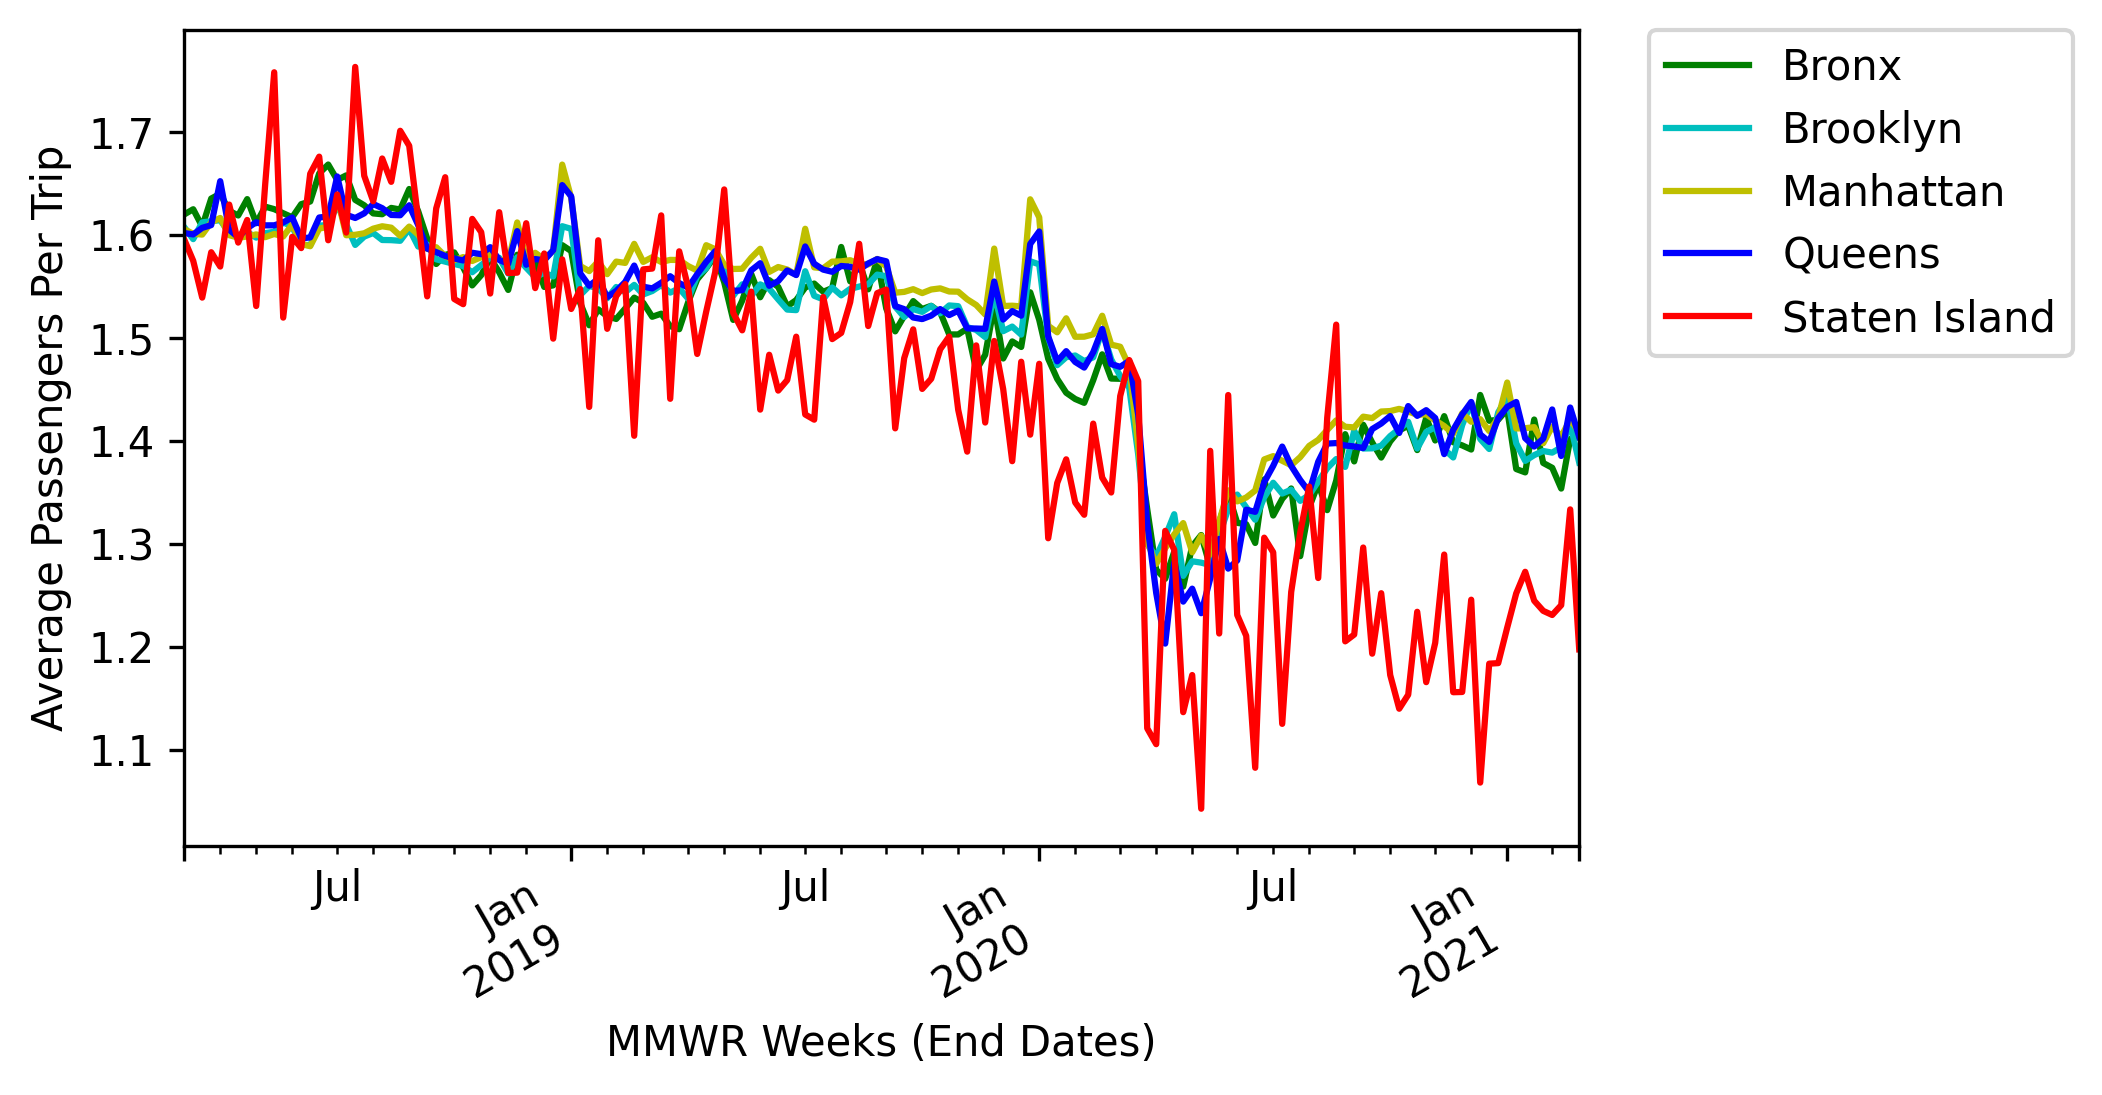
\includegraphics[width=0.45\textwidth]{../plots/time-series-Average Passengers Per Trip-vs-MMWR Weeks (End Dates)-by-do_borough.png}
    %     % this ensures your figures are centered where possible
    %     \centering
    %     \caption{How average passenger counts per week per pickup borough vary over time.} % refer to this image as (Figure 1)
    %     \label{fig:ts-pass-count-weeks}
    % \end{figure}
% \end{multicols}

% \begin{figure}[h]
%     % change the scale multiplier to make the figures smaller or larger
%     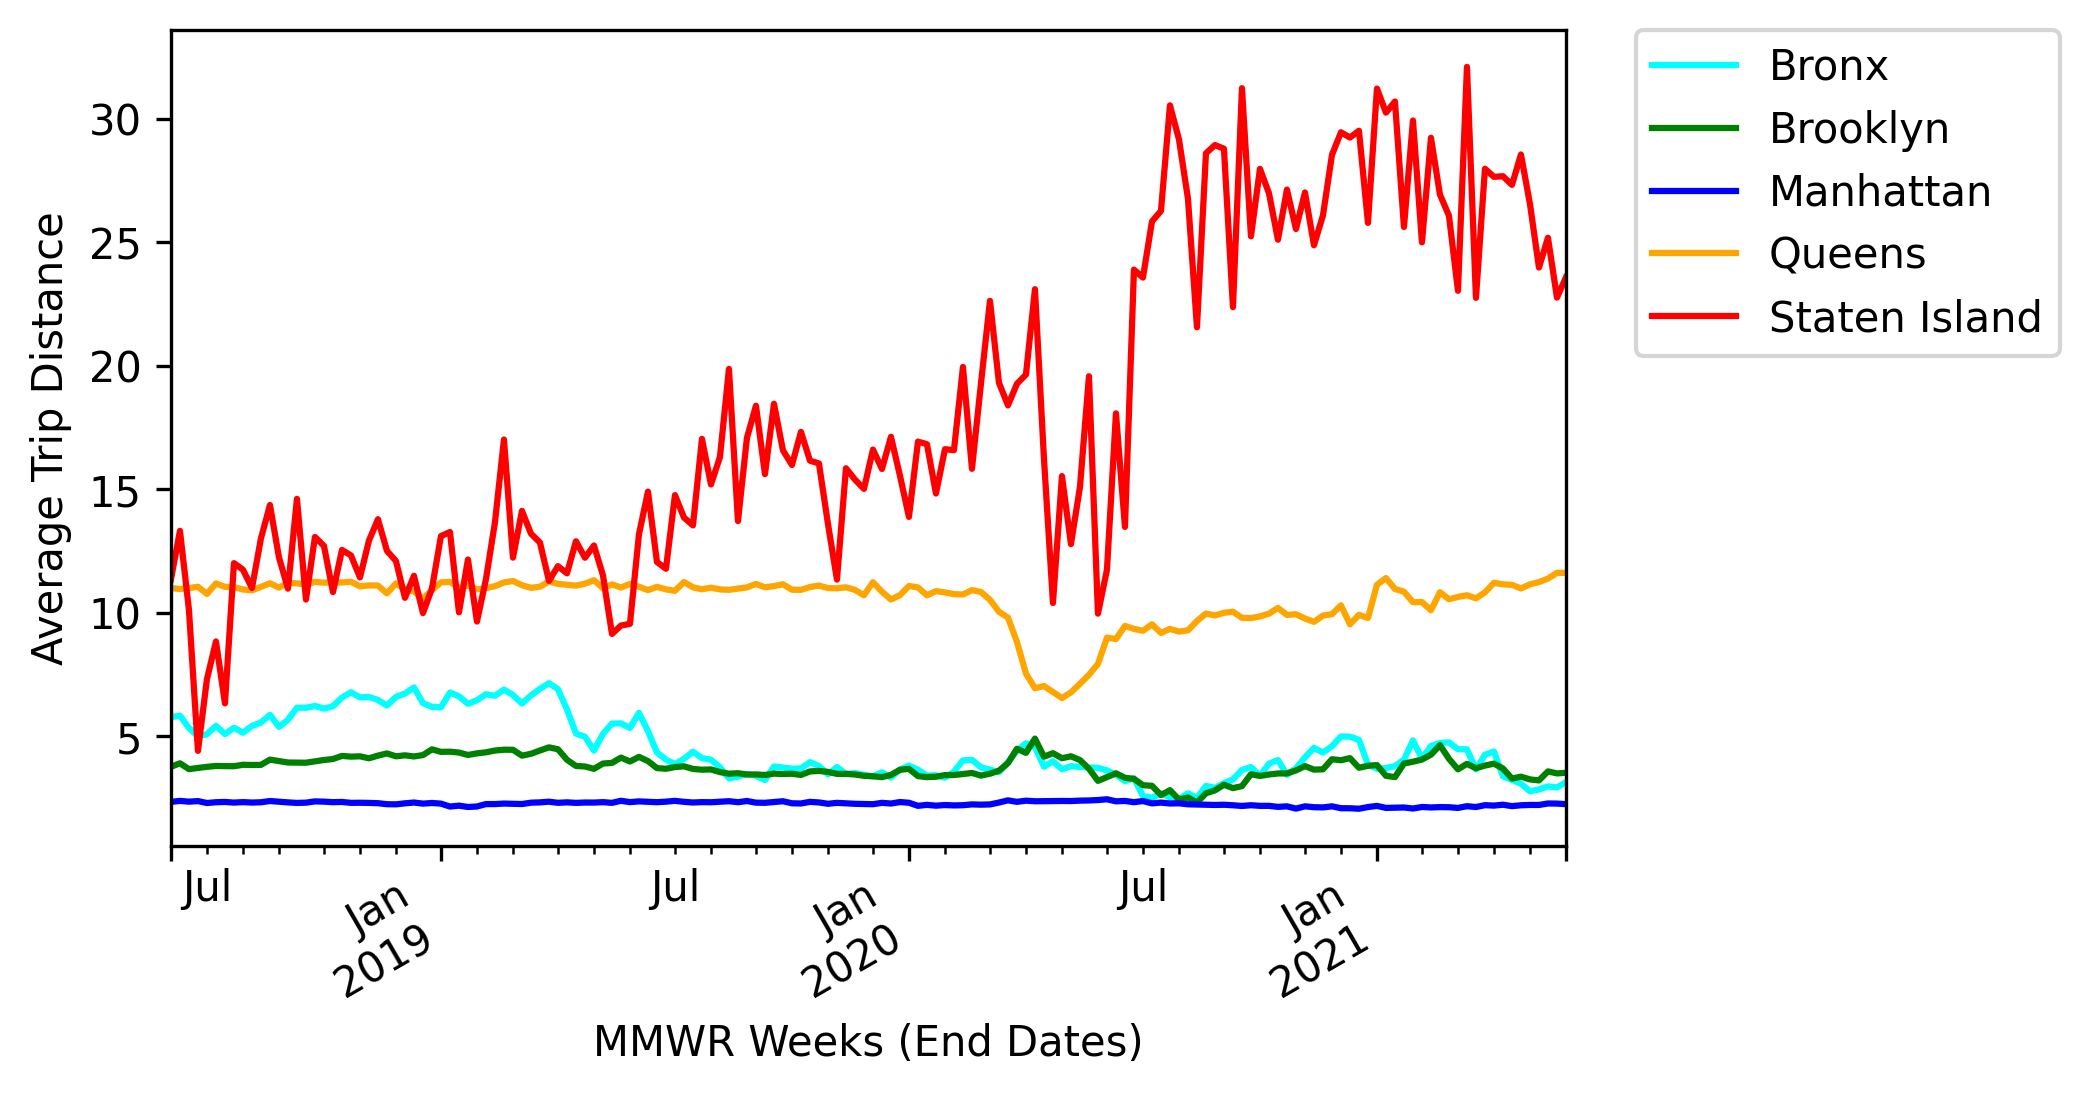
\includegraphics[width=0.45\textwidth]{../plots/time-series-Average Trip Distance-vs-MMWR Weeks (End Dates)-by-pu_borough.png}
%     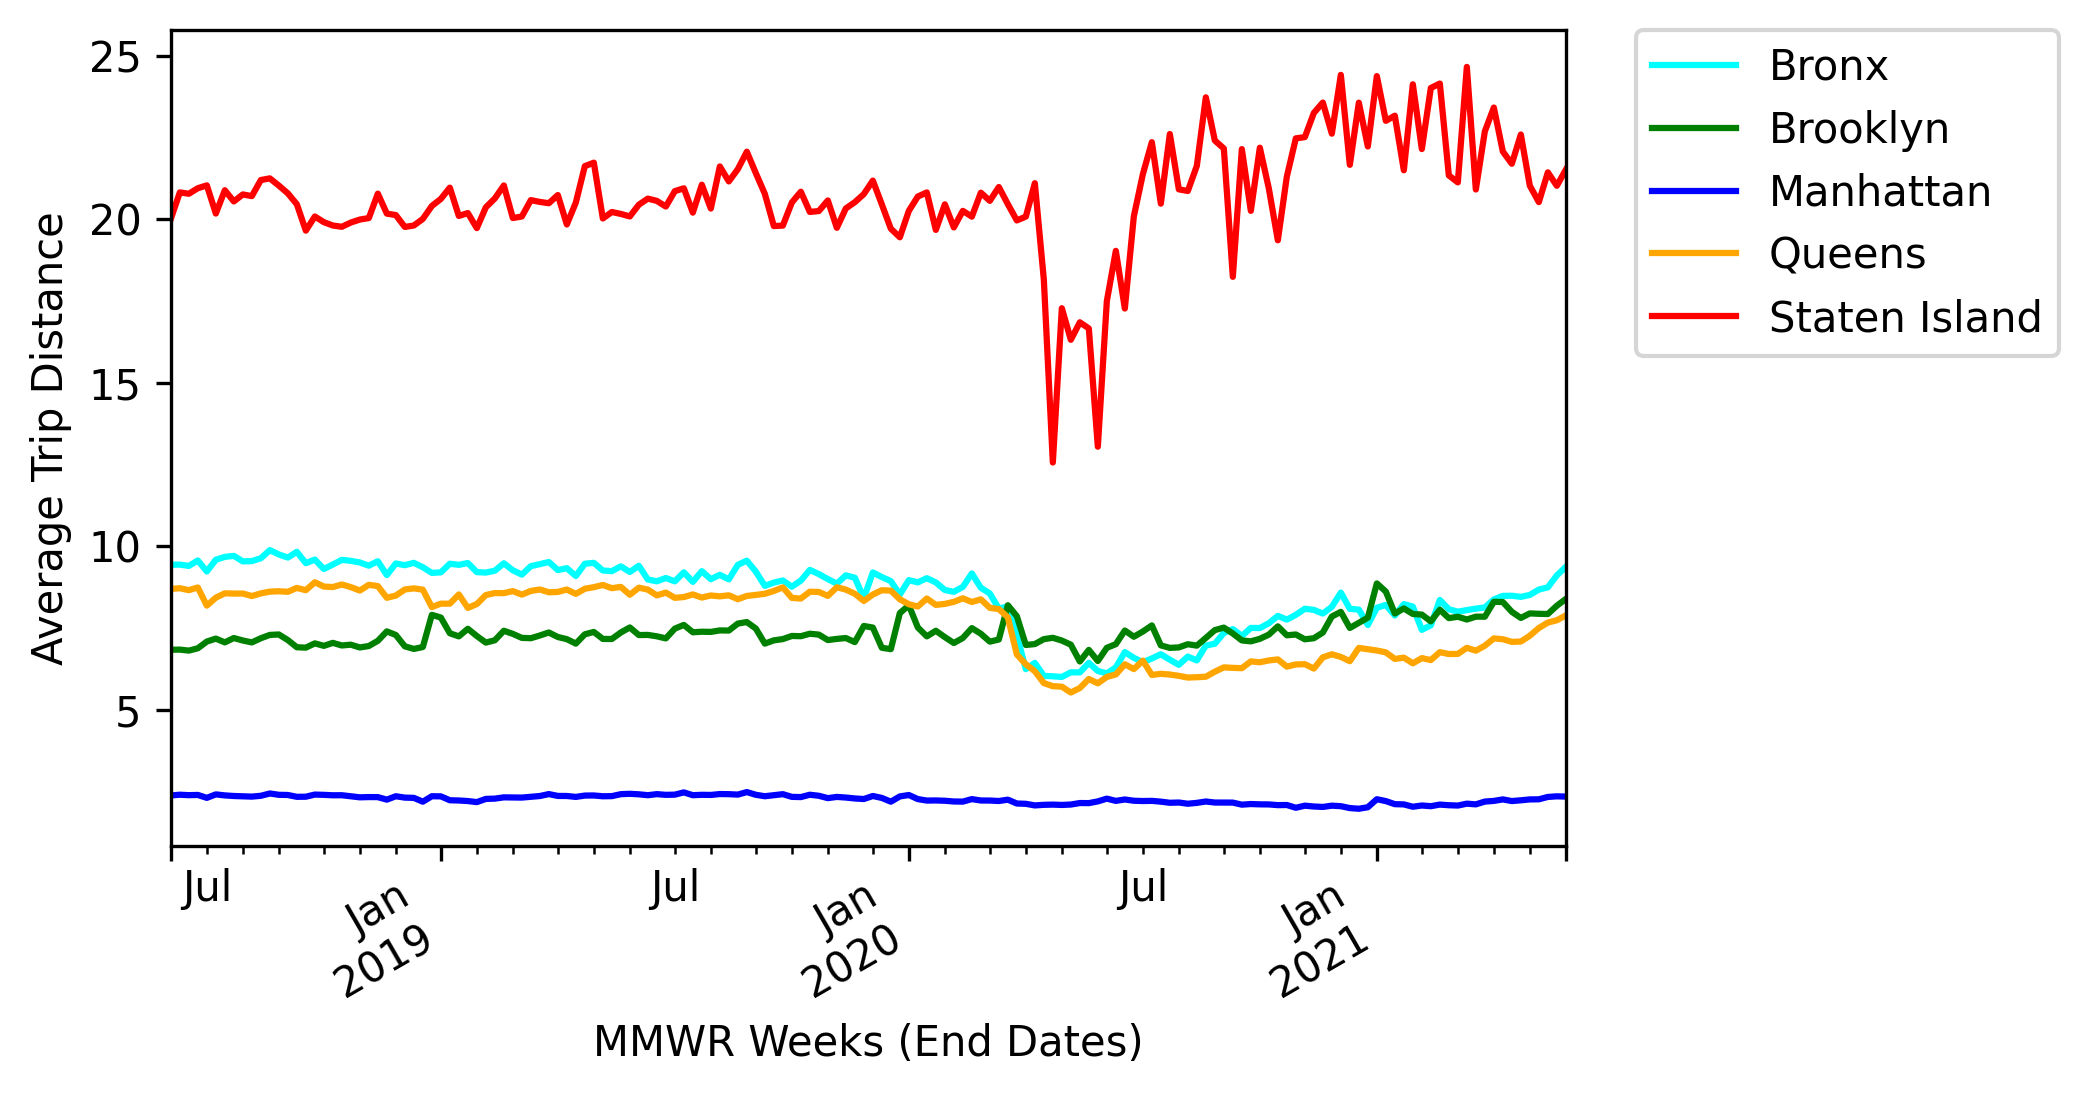
\includegraphics[width=0.45\textwidth]{../plots/time-series-Average Trip Distance-vs-MMWR Weeks (End Dates)-by-do_borough.png}
%     % this ensures your figures are centered where possible
%     \centering
%     \caption{How average trip distances per week per pickup (left) and dropoff (right) borough vary over time.} % refer to this image as (Figure 1)
%     \label{fig:ts-dist-weeks}
% \end{figure}

This uptick in travel distance is likely caused by reduced usage of the Staten Island ferry and the reduced schedule during the pandemic \cite{dot2020}.
If this is the case, then Figure~\ref{fig:ts} suggests that people travelling to and from Staten Island rely on taxis to be safer and ontime over the ferry service.
The trip distances between boroughs are generally not very homoegeneous. 
A likely reason for this heterogeneity is the difference in commutes to work, since
many jobs are likely located in Manhattan.

It appears as though passenger counts experience more drastic variation week-on-week.
The greatest instability in passenger counts appears to come from trips going to or from Staten Island,
while travel to or from other boroughs appears more stable and similar week-on-week. 
This may also come as a result of Staten Island's separation from the other boroughs,
however a true cause and effect relationship on this phenomenon would require a properly designed experiment to confirm.

% \begin{figure}[h]
%     % change the scale multiplier to make the figures smaller or larger
%     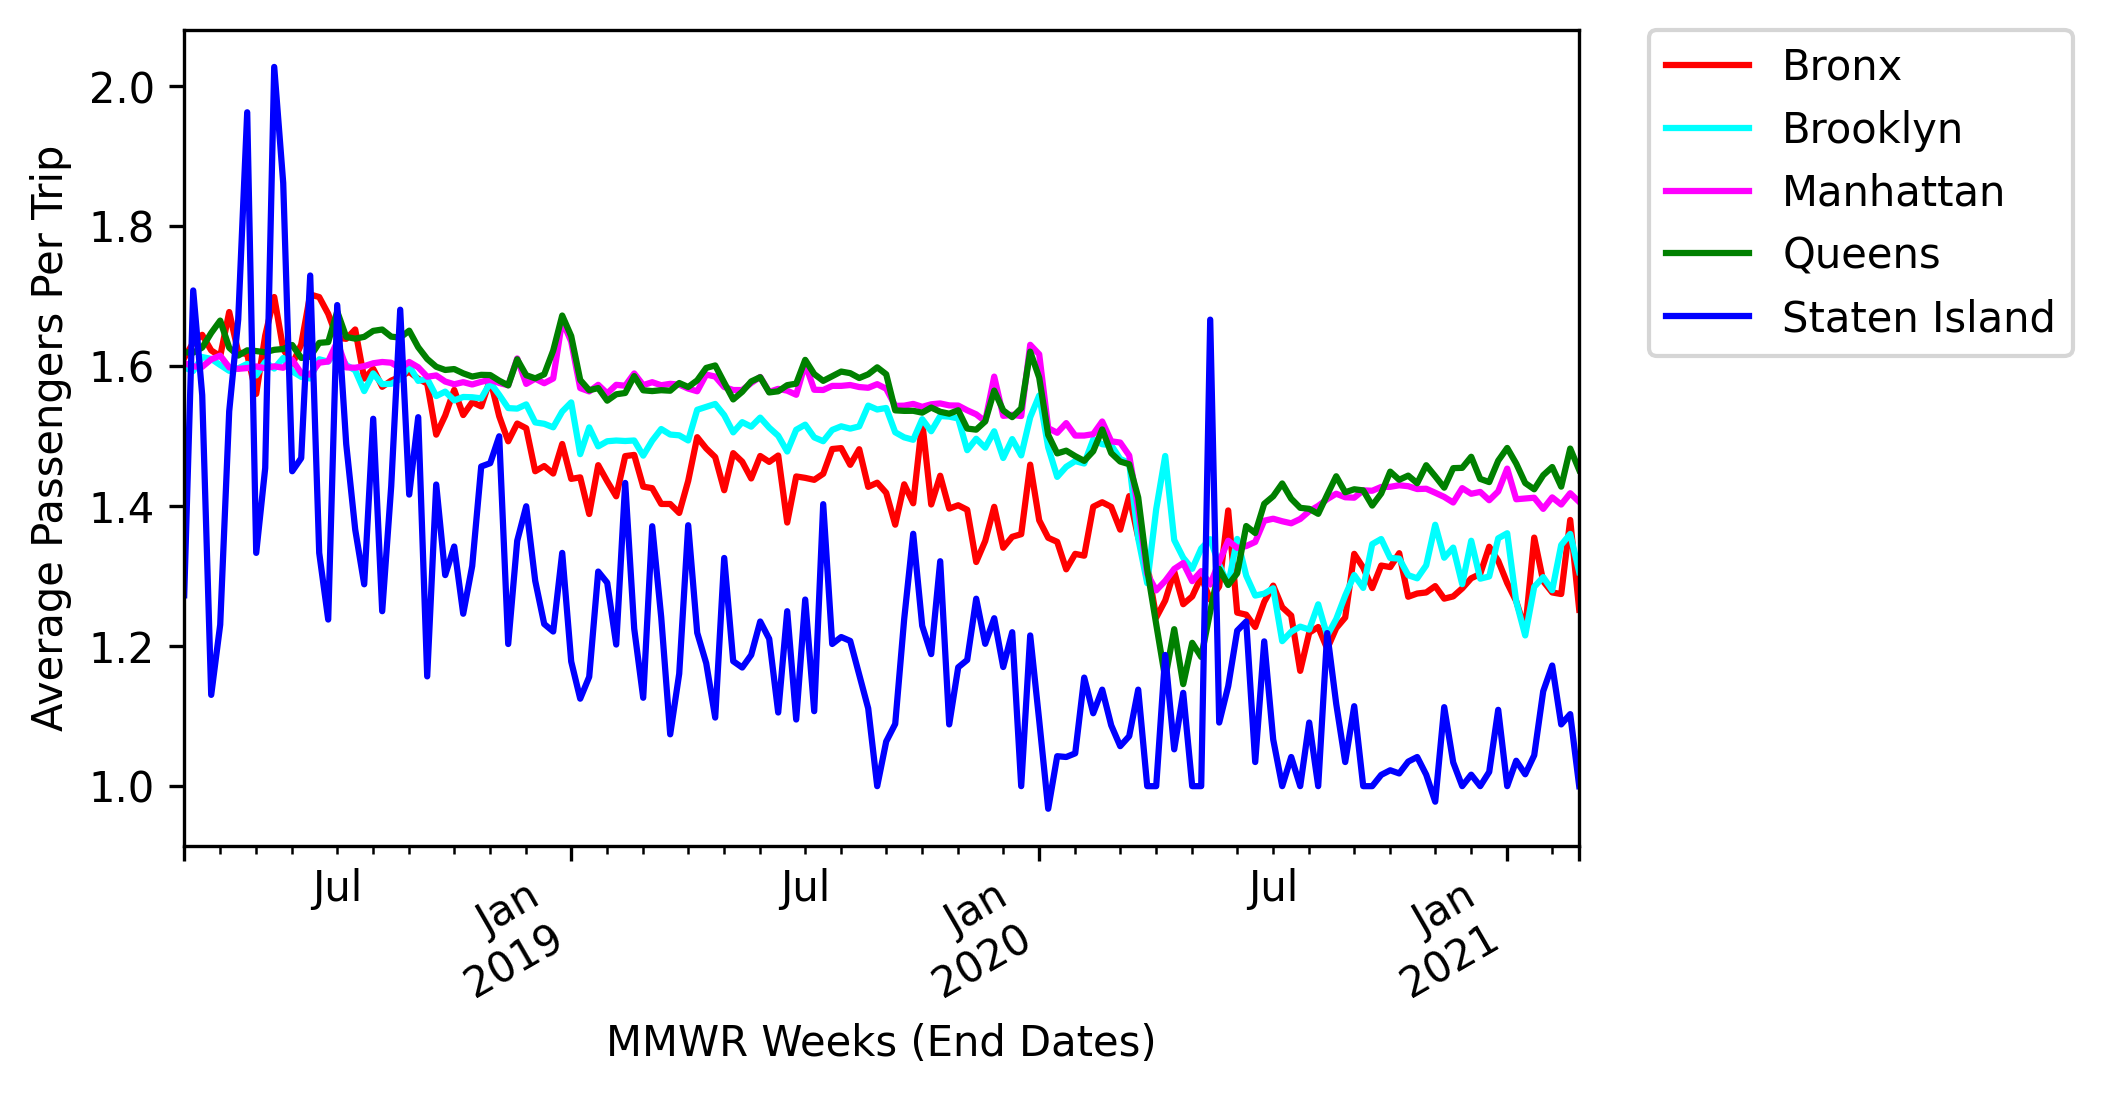
\includegraphics[width=0.45\textwidth]{../plots/time-series-Average Passengers Per Trip-vs-MMWR Weeks (End Dates)-by-pu_borough.png}
%     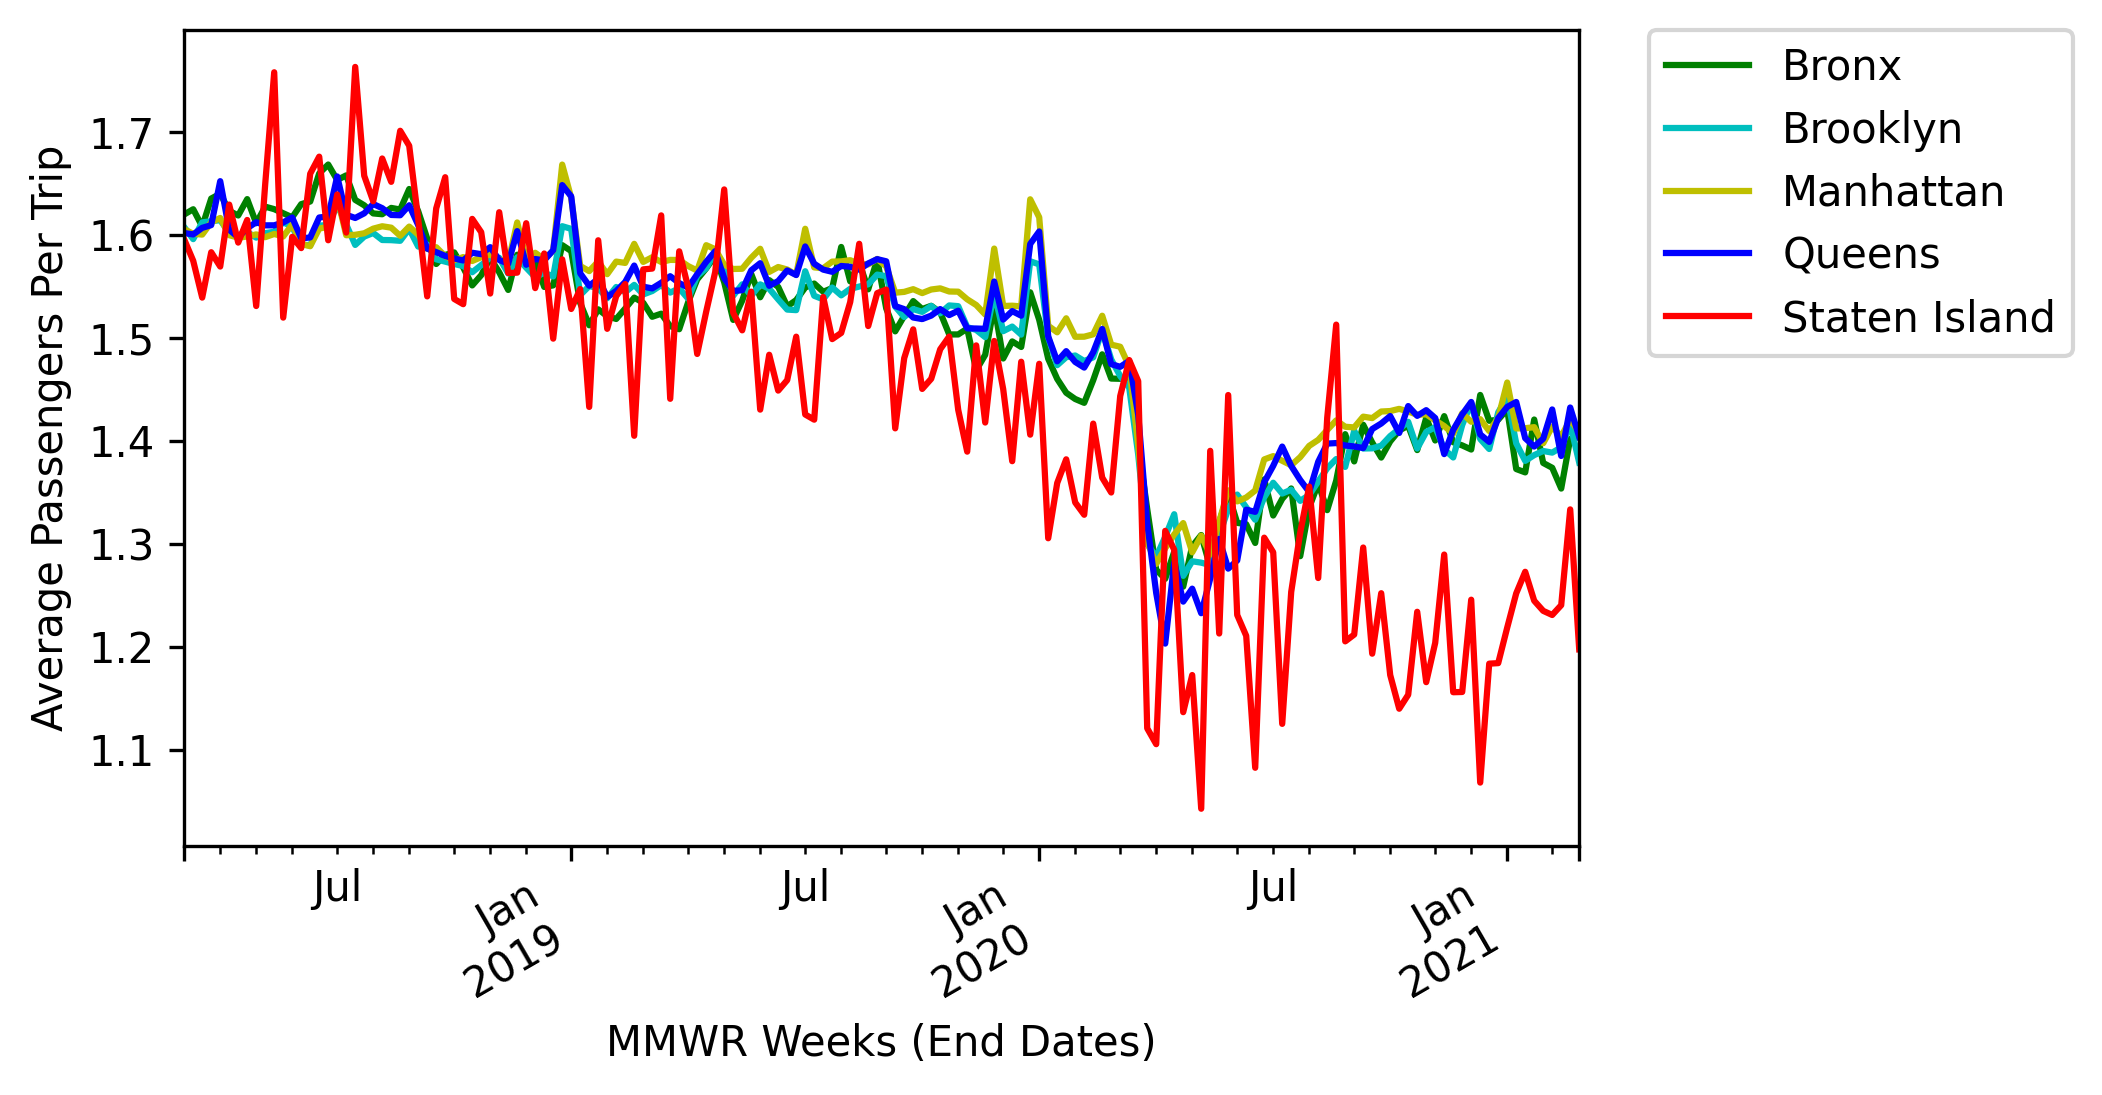
\includegraphics[width=0.45\textwidth]{../plots/time-series-Average Passengers Per Trip-vs-MMWR Weeks (End Dates)-by-do_borough.png}
%     % this ensures your figures are centered where possible
%     \centering
%     \caption{How average passenger count per week per pickup (left) and dropoff (right) borough vary over time.} % refer to this image as (Figure 1)
%     \label{fig:ts-pass-count-weeks}
% \end{figure}


% \begin{figure}[H]
%     % change the scale multiplier to make the figures smaller or larger
%     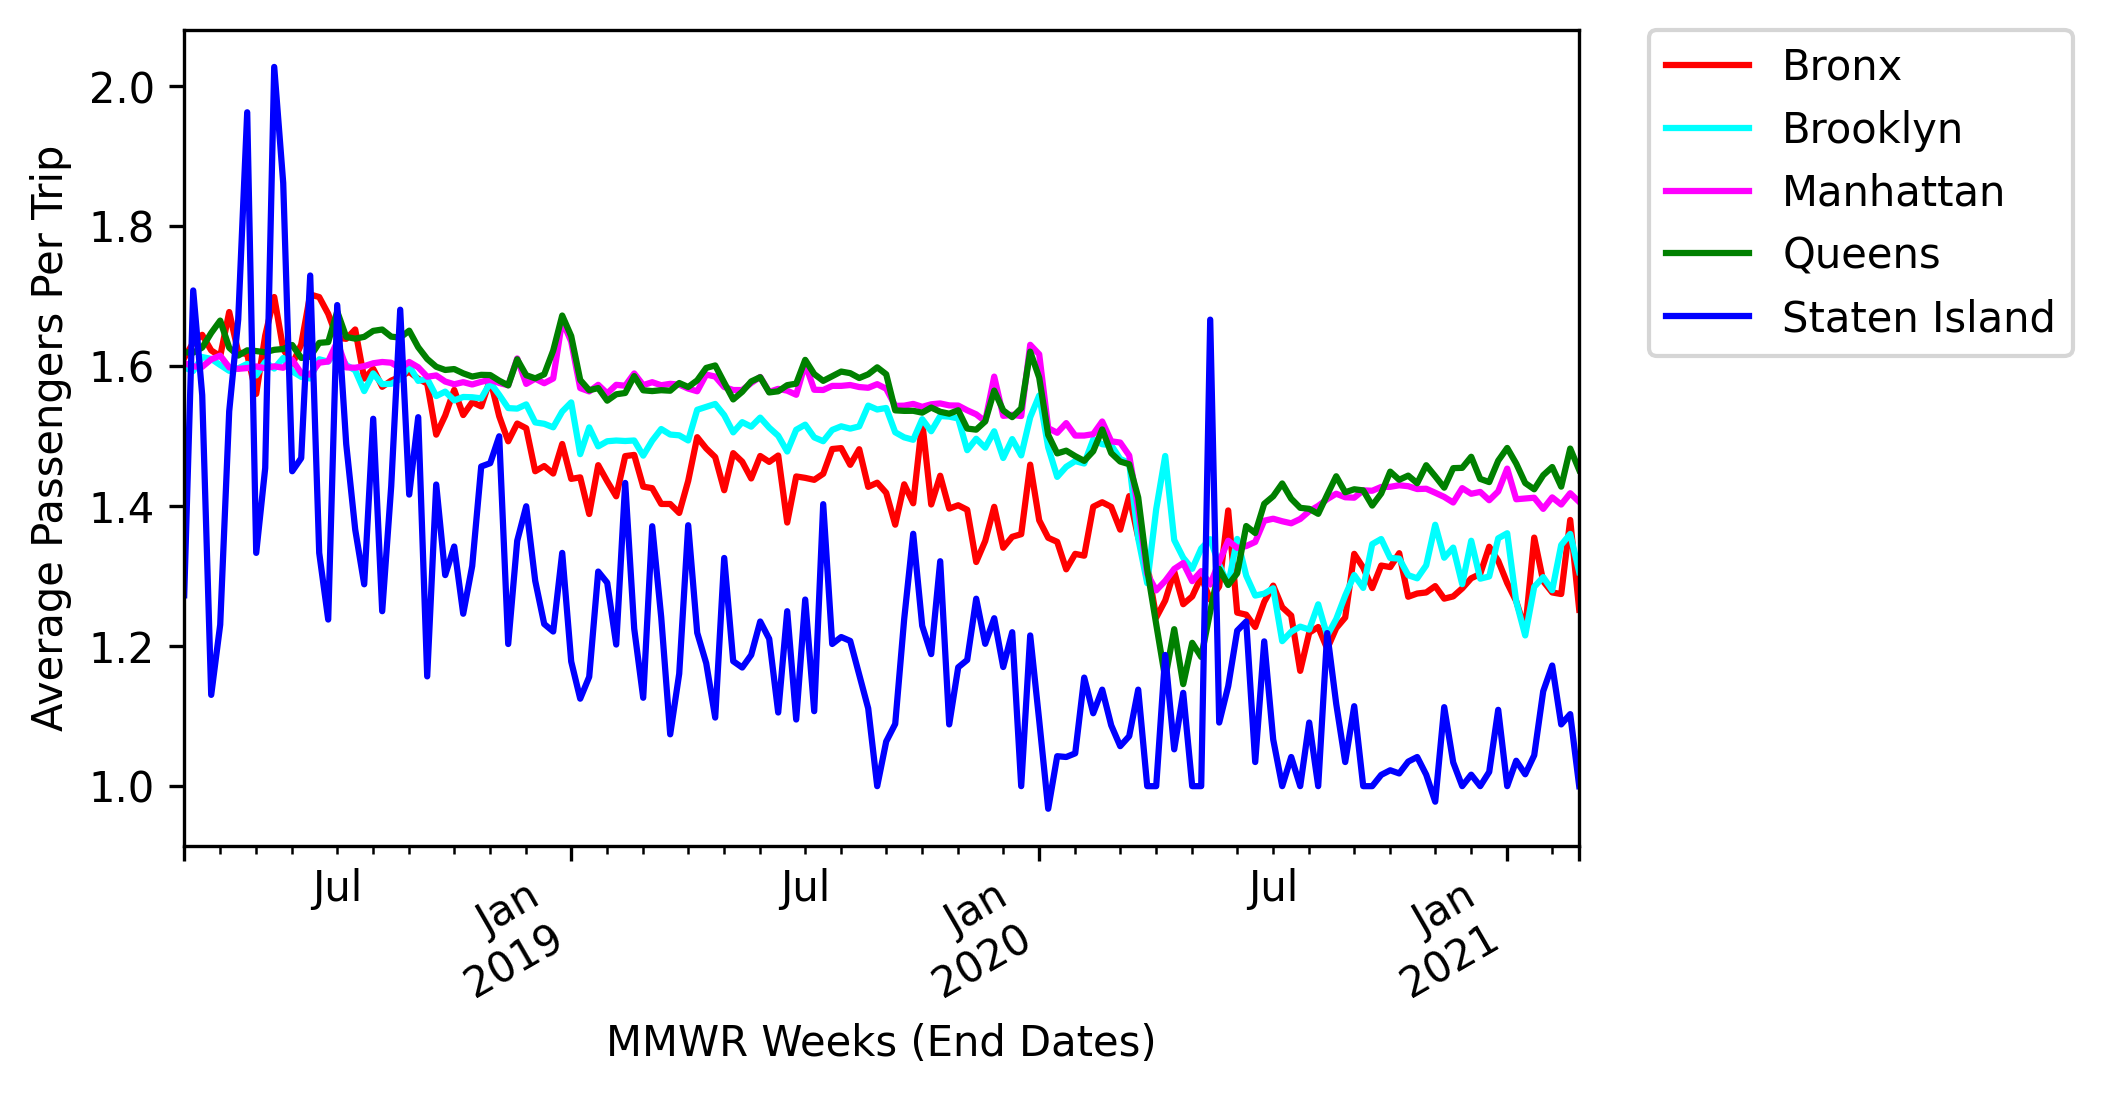
\includegraphics[width=0.5\textwidth]{../plots/time-series-Average Passengers Per Trip-vs-MMWR Weeks (End Dates)-by-pu_borough.png}
%     % 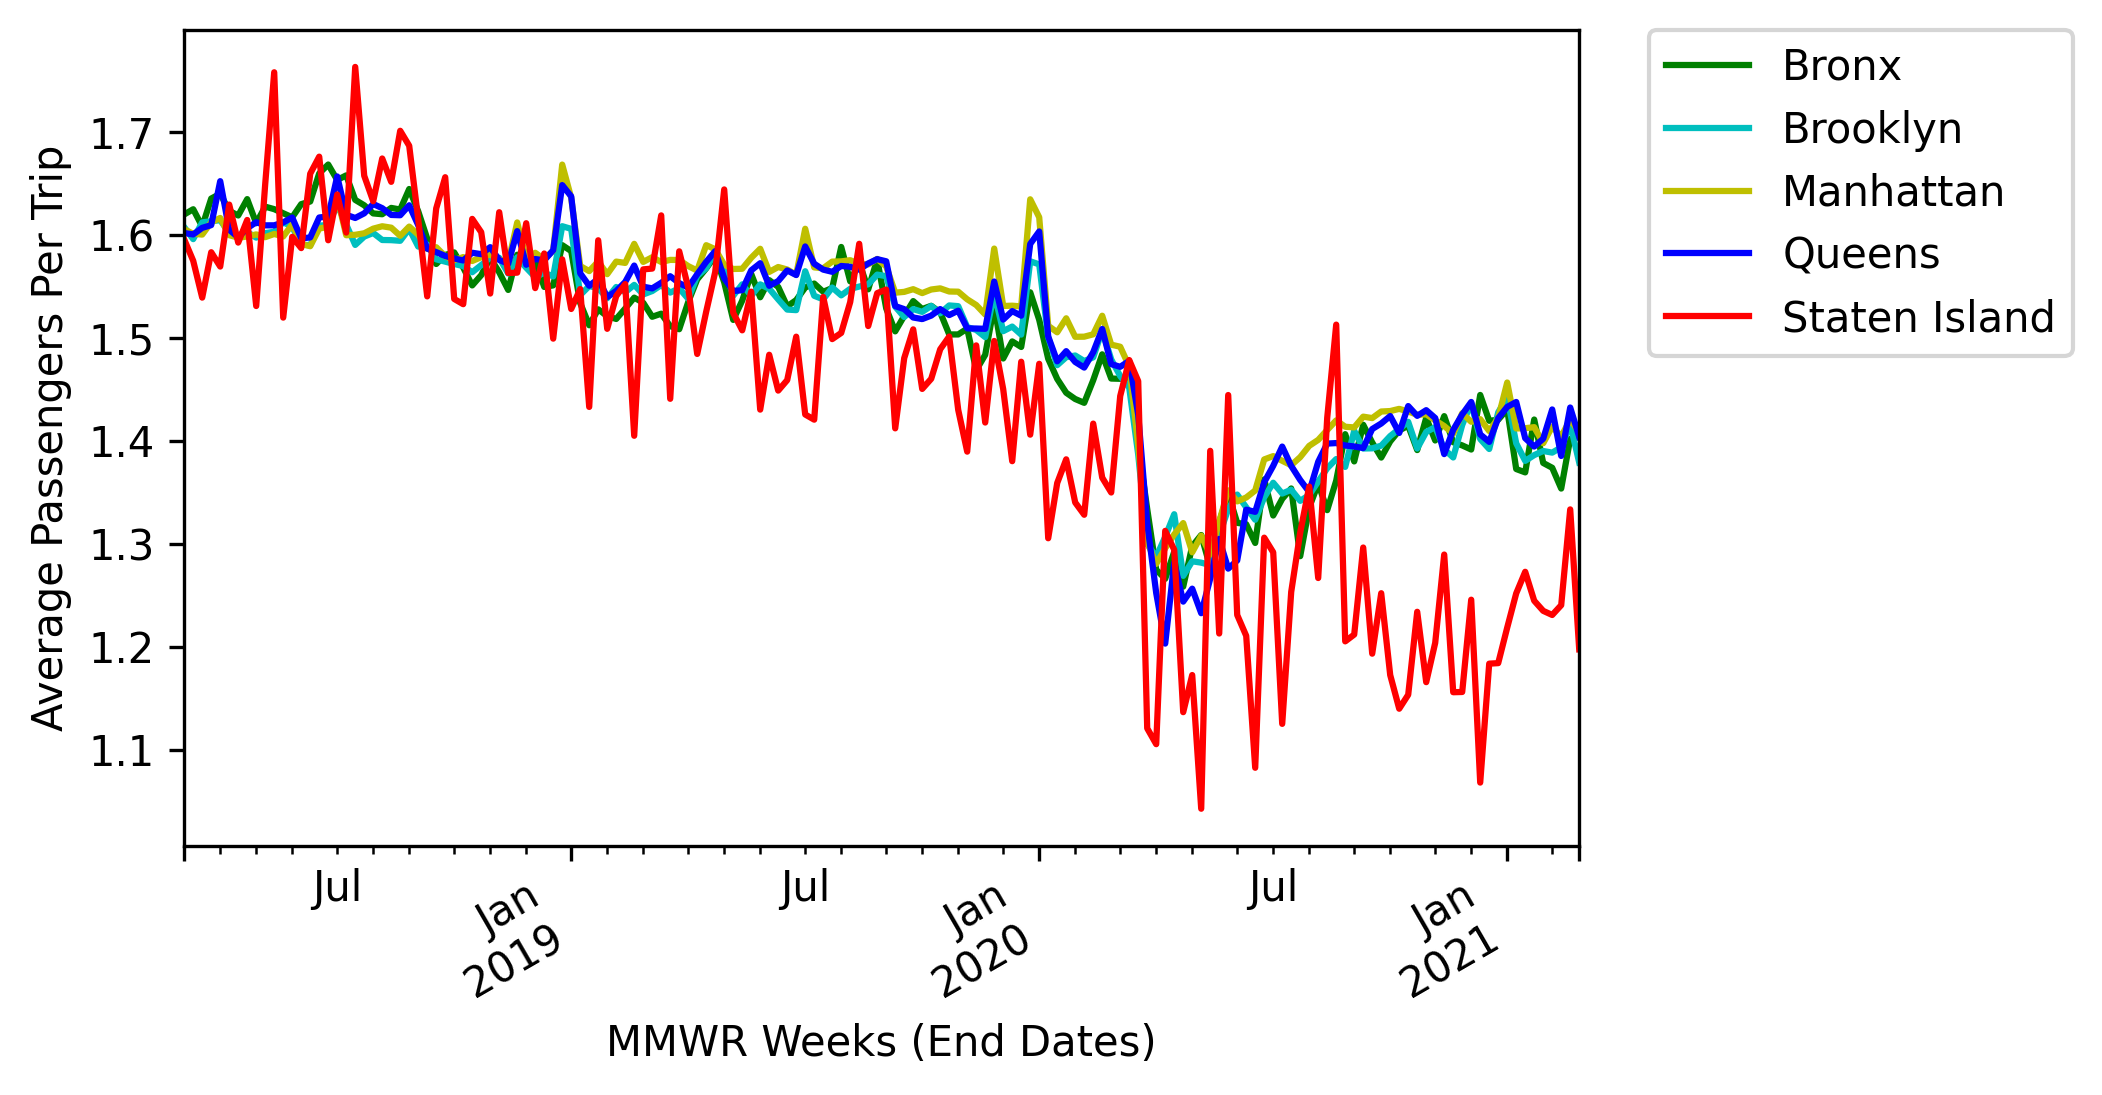
\includegraphics[width=0.45\textwidth]{../plots/time-series-Average Passengers Per Trip-vs-MMWR Weeks (End Dates)-by-do_borough.png}
%     % this ensures your figures are centered where possible
%     \centering
%     \caption{How average passenger counts per week per pickup borough vary over time.} % refer to this image as (Figure 1)
%     \label{fig:ts-pass-count-weeks}
% \end{figure}
    \textbf{Geospatial Visualisation:}
While time series plots display variation in average trip distance over time, 
they do not clearly convey the meaning of these differences.
Figures~\ref{map:overall} and \ref{maps} compares the average trip radius overall, 
the average trip radius for the week with maximum COVID-19 cases per capita, 
and the week with maximum Influenza cases per capita per pickup borough.

\begin{multicols}{2}
\begin{figure}[H]

    % this ensures your figures are centered where possible
    \centering

    % change the scale multiplier to make the figures smaller or larger
    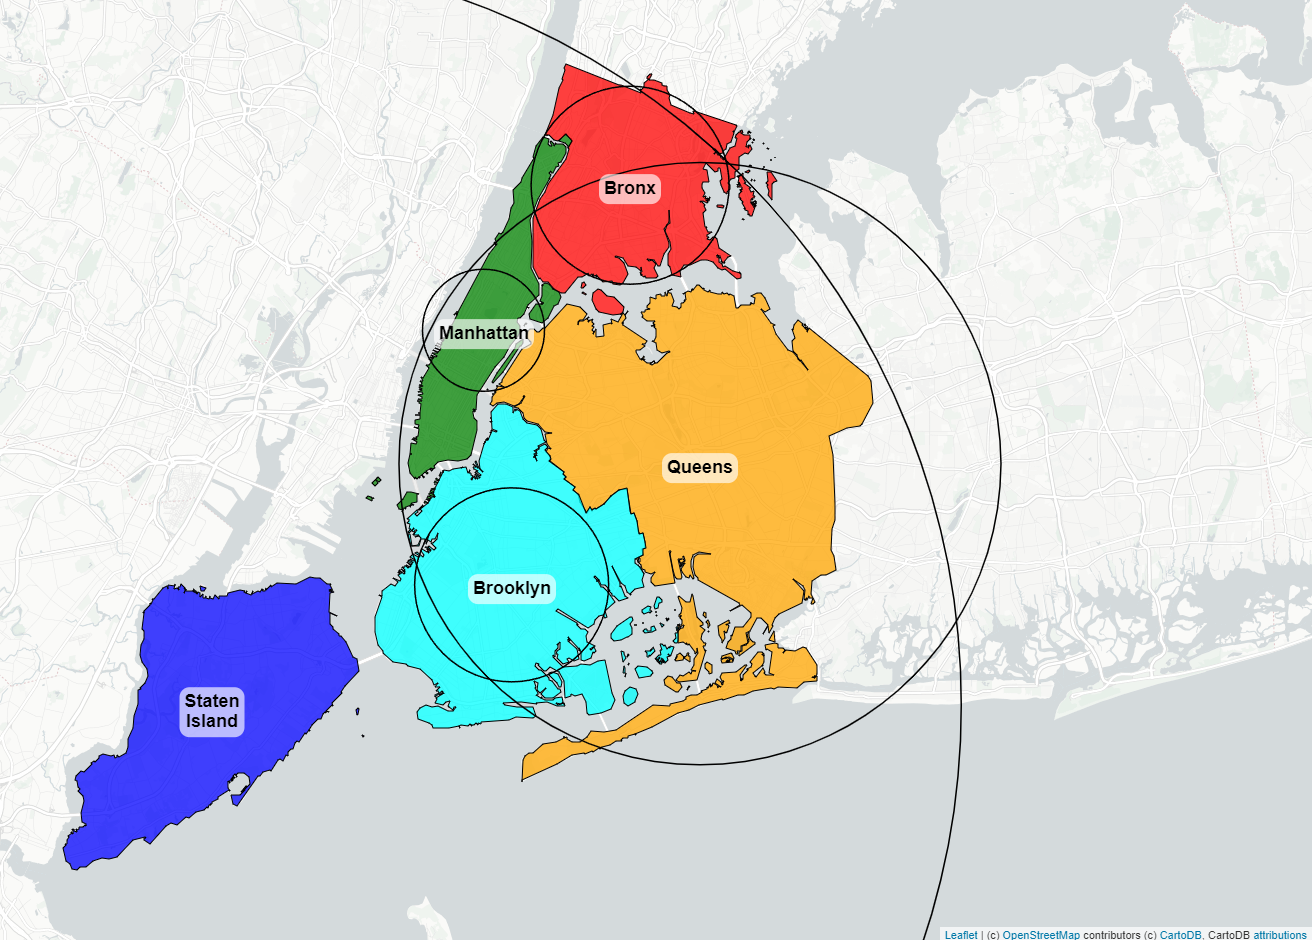
\includegraphics[width=0.5\textwidth]{../plots/map-avg-trip-distance-overall-pu_borough-MODIFIED.png}

    \caption{Map of average trip distance over Timeline 2.} 
    % refer to this image as (Figure 1)
    \label{map:overall}
\end{figure}

At a first glance, Staten Island appears to experience the most change in trip distance during times of high case rates.
While the initial expectation is that trip distances will decrease following weeks with many virus cases,
the reliance on taxis starting in Staten Island also depends on the type of virus.
Following maximum COVID-19 cases, the average trip radius is wider, 
whereas following maximum Influenza cases, the average trip radius is more constricted.
This suggests that there are different reactions to the prevalence of different viruses.
An alternative explanation is that the Staten Island ferry may have been fully operational when the borough experienced its maximum Influenza case rate.

The other boroughs do not vary as significantly in trip distance.
This may be due to their proximity to each other.
Another contributing factor could be the generally larger populations of these boroughs,
meaning that a larger proportion of people are unlikely to change their taxi usage based on outside factors.


\end{multicols}

% \begin{figure}[H]

%     % this ensures your figures are centered where possible
%     \centering

%     % change the scale multiplier to make the figures smaller or larger
%     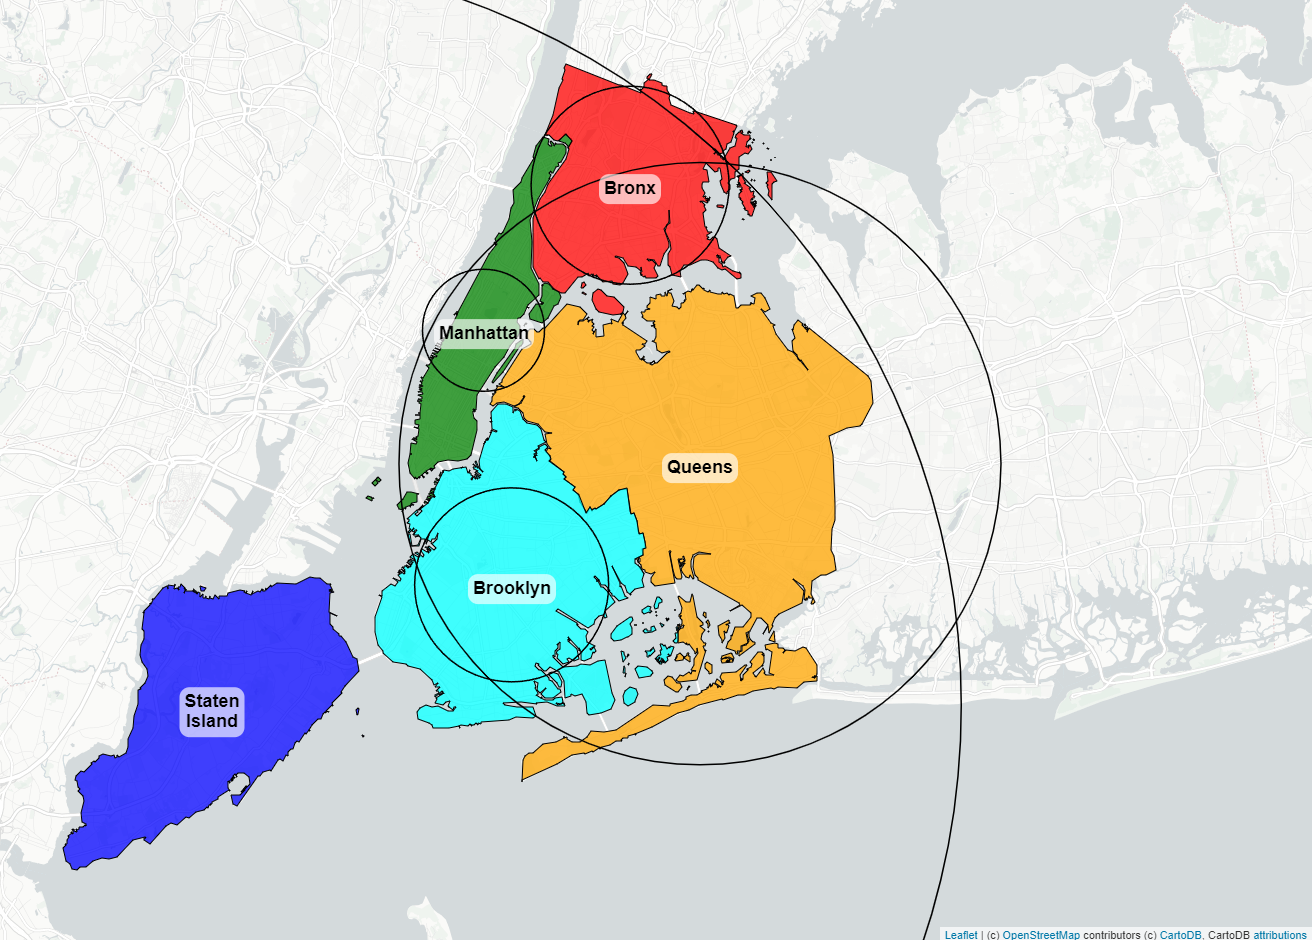
\includegraphics[width=0.45\textwidth]{../plots/map-avg-trip-distance-overall-pu_borough-MODIFIED.png}

%     \caption{Map of average trip distance over Timeline 2.} 
%     % refer to this image as (Figure 1)
%     \label{map:overall}
% \end{figure}

% \pagebreak

% \begin{multicols}{2}
    \begin{figure}[H]

        % this ensures your figures are centered where possible
        \centering
    
        % change the scale multiplier to make the figures smaller or larger
        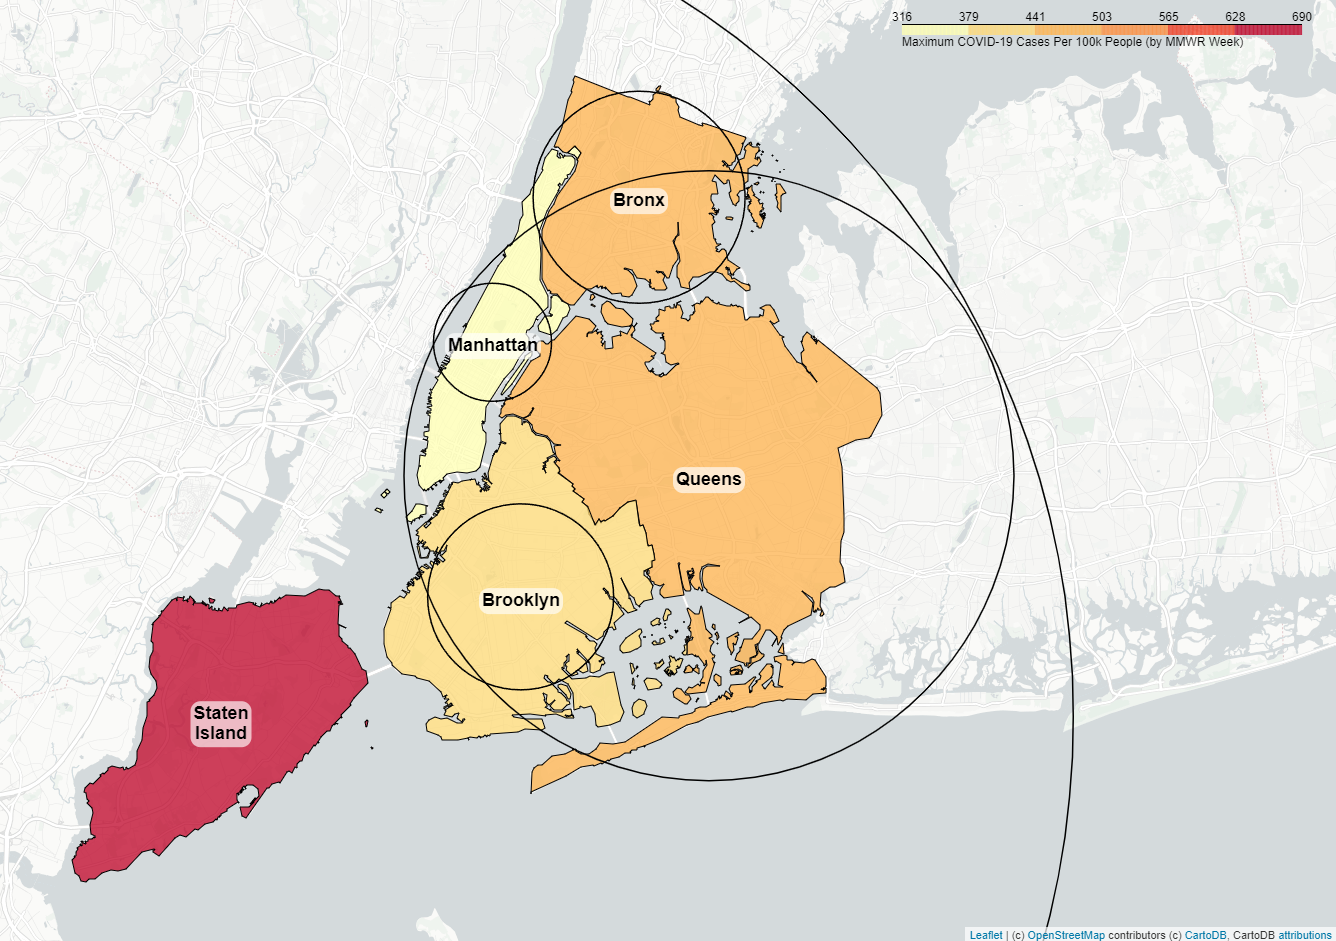
\includegraphics[width=0.45\textwidth]{../plots/map-avg-trip-distance-at-max-covid-by-pu_borough-MODIFIED.png}
        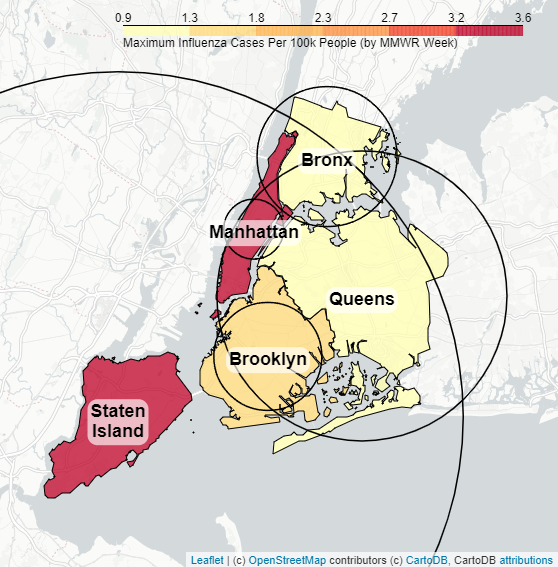
\includegraphics[width=0.45\textwidth]{../plots/map-avg-trip-distance-at-max-flu-by-pu_borough-MODIFIED.png}

        \caption{Map of weekly average trip distance following the maximum COVID-19 (left) and Influenze (right) cases rate over Timeline 2.} % refer to this image as (Figure 1)
        \label{maps}
    \end{figure}
    
    % \begin{figure}[H]
    
    %     % this ensures your figures are centered where possible
    %     \centering
    
    %     % change the scale multiplier to make the figures smaller or larger
    %     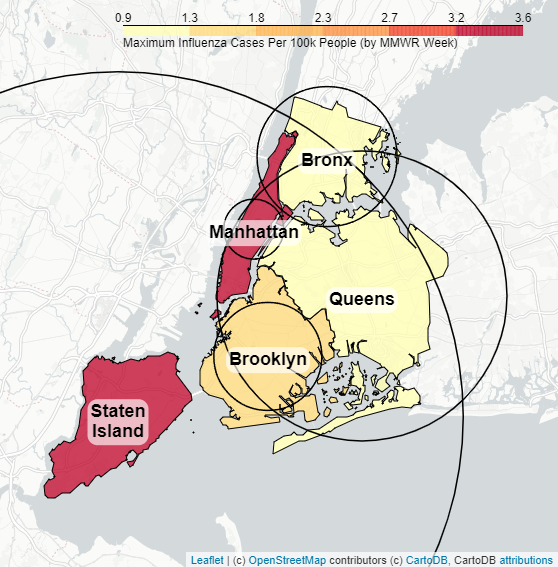
\includegraphics[width=0.45\textwidth]{../plots/map-avg-trip-distance-at-max-flu-by-pu_borough-MODIFIED.png}
    
    %     \caption{Map of weekly average trip distance following the maximum Influenza cases rate over Timeline 2.} % refer to this image as (Figure 1)
    %     \label{map:flu}
    % \end{figure}    
% \end{multicols}


\textbf{Distributions:} 
It is important to note that both average trip distances and passenger counts 
are random variables with different properties, and are therefore modelled using different distributions.
Trip distances are a continuous metric, while passenger counts are discrete, but neither can be negative.
This means that two different forms of linear model are used to model each measure.

\begin{figure}[H]
    % change the scale multiplier to make the figures smaller or larger
    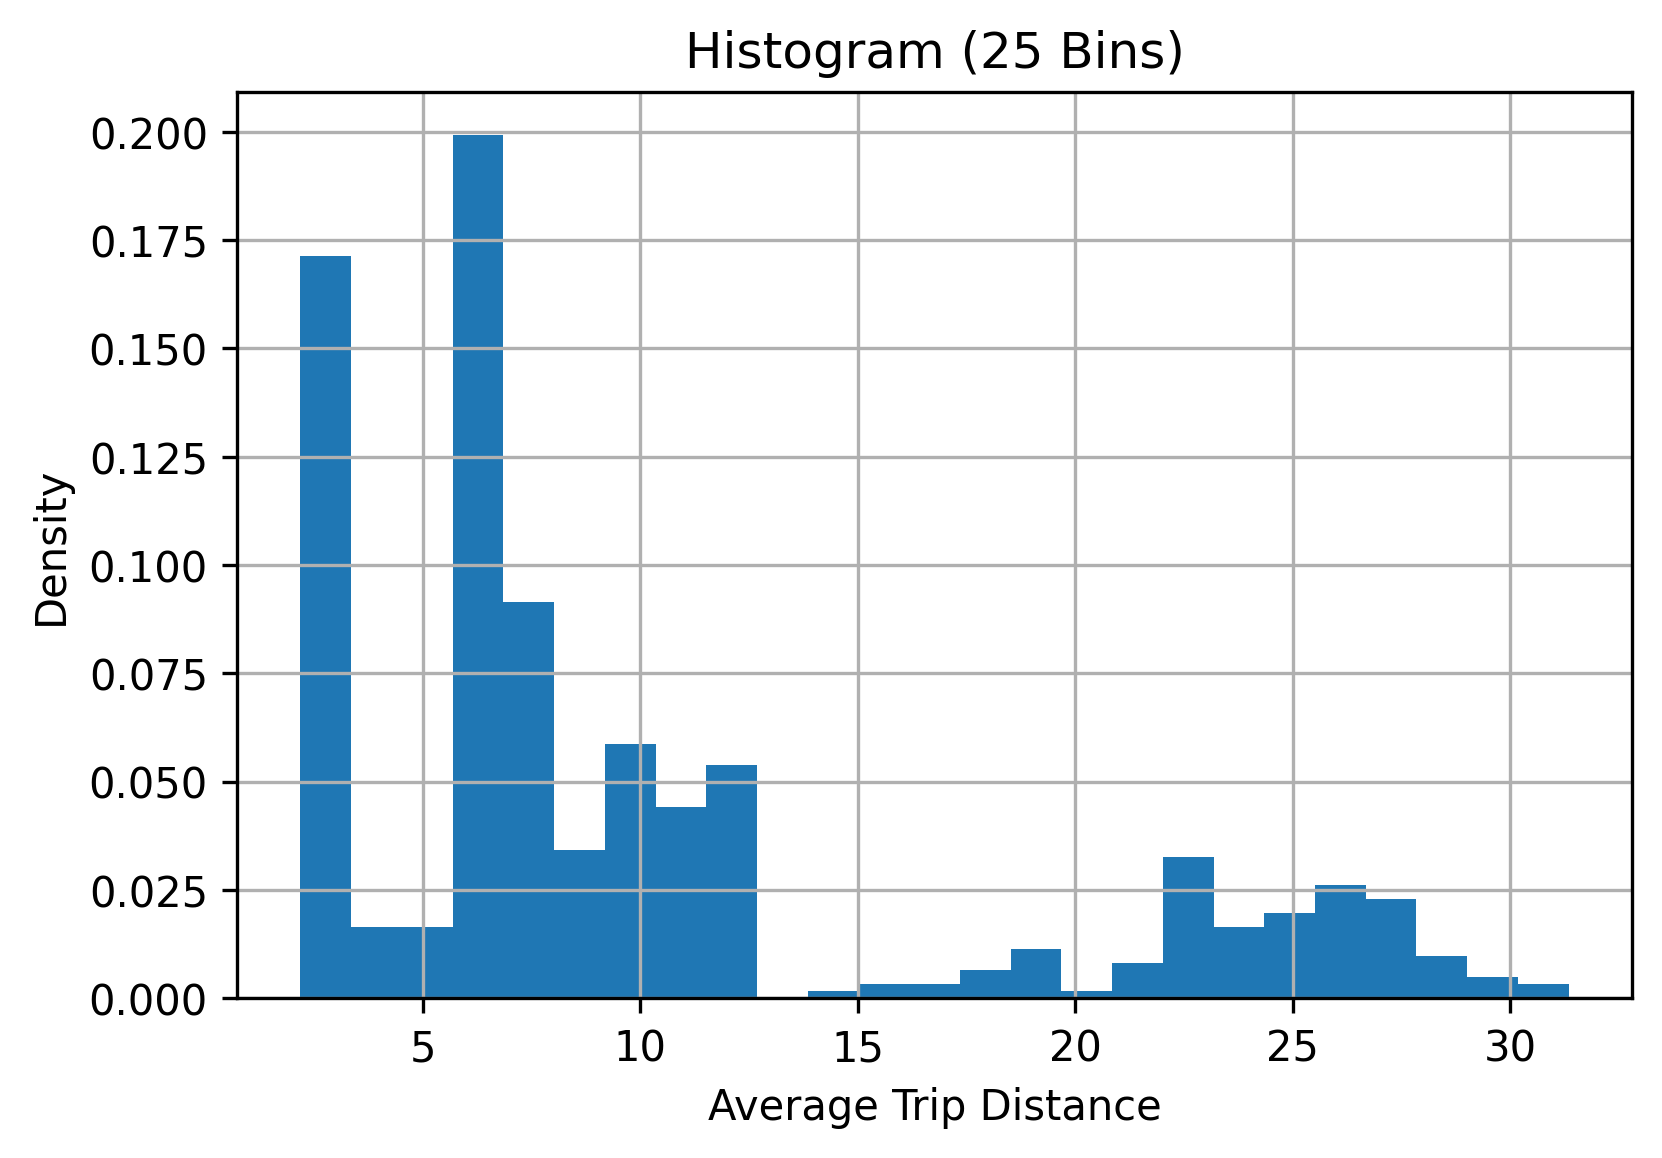
\includegraphics[width=0.40\textwidth]{../plots/histogram-Average Trip Distance-25-bins.png}
    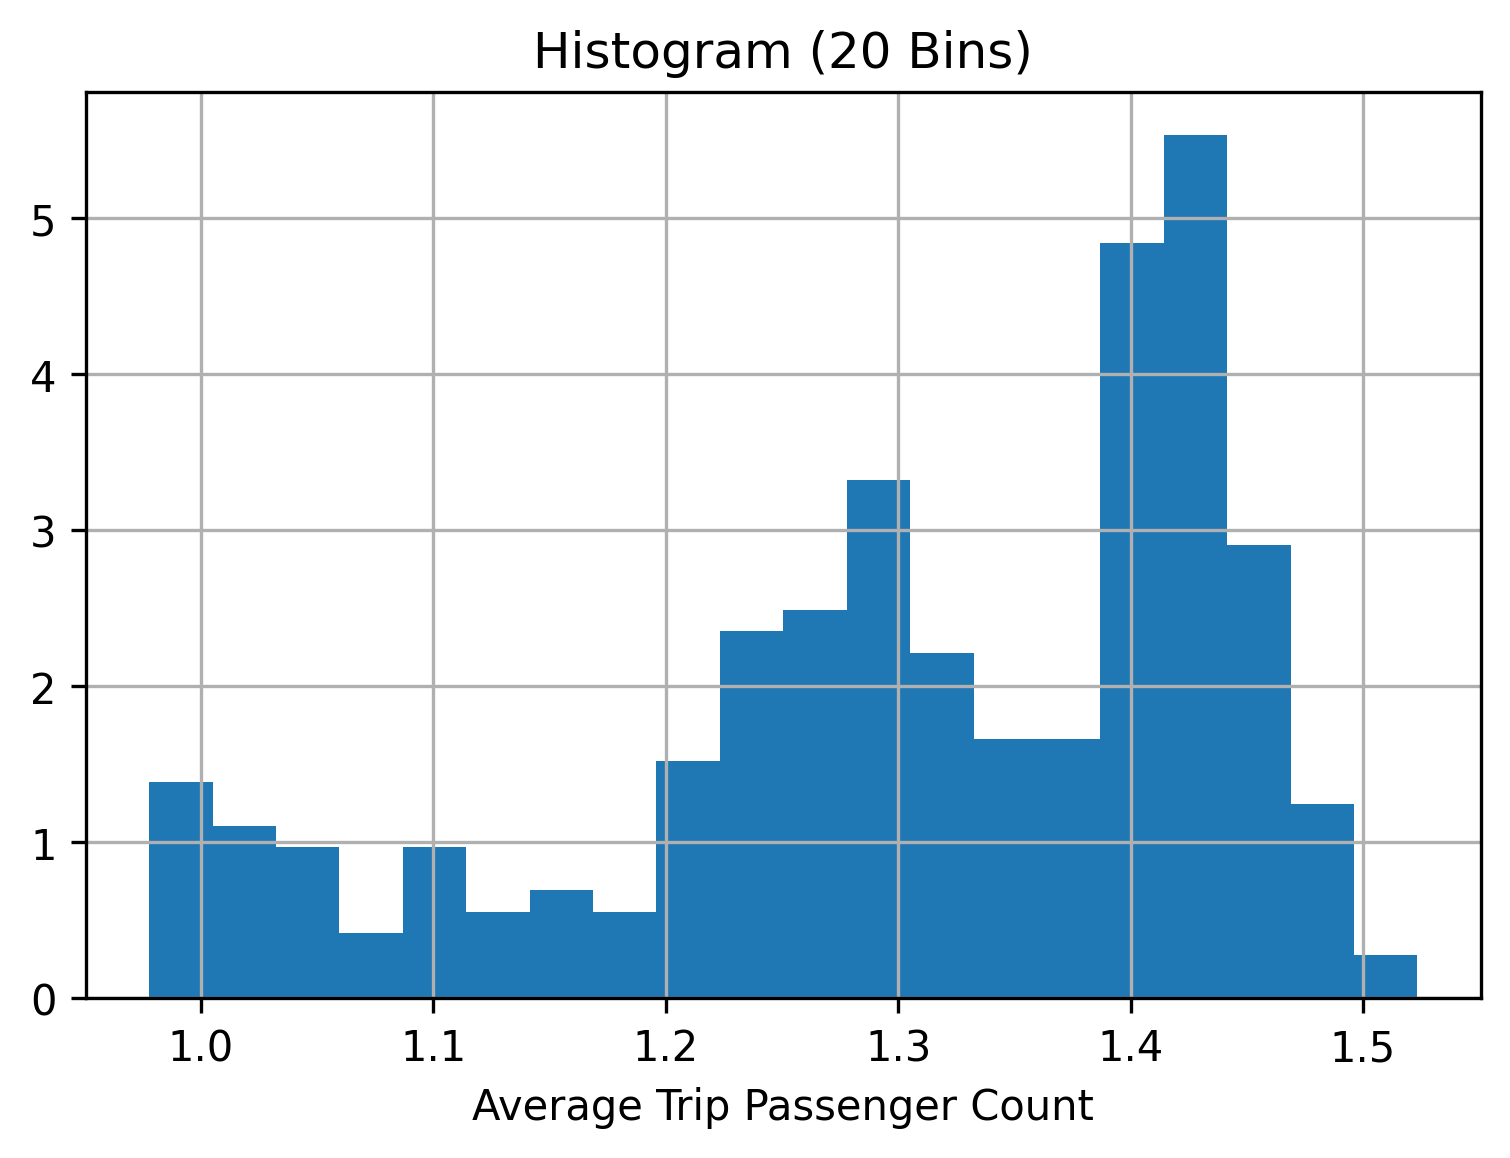
\includegraphics[width=0.38\textwidth]{../plots/histogram-Average Trip Passenger Count-20-bins.png}
    % this ensures your figures are centered where possible
    \centering
    \caption{Probability density histogram of average trip distance (left) and average trip passenger count (right) over Timeline 2.} % refer to this image as (Figure 1)
    \label{fig:hists}
\end{figure}

The selected reliance measures have different properties and distributions.
While the passenger count represents a discrete measure, trip distance is measured on a continuous scale.
The weekly average trip distances have an overall average of $9.379$ miles, with a variance of $88.41$.
Such a wide variance suggests that trip distances have a somewhat wide distribution.
According to Figure~\ref{fig:hists}, there appear to be three distinct peaks in trip distance,
each approximately normally distributed. 
Earlier evidence of positively skewed distribution occurs in Figure~\ref{fig:ts}, 
where there are three distinct bands of trip distance when grouped by borough.
The weekly average passenger counts have an overall average of $1.307$ with a variance of $0.01861$.
Such a low variance appears to contradict what is shown in Figure~\ref{fig:ts}.
This suggests that boroughs are a confounding factor in passenger counts.
Due to this measure being discrete, it is best described by a binomial distribution with a negative skew.

\subsubsection{Modelling}

Both borough and time appear to affect the selected measures of reliance,
meaning that they both need to be considered in the generated models.
This means that for each week's average reliance measure, 
a linear model is generated with the predictors: 
borough,
the preceding week's index in the timeline,
the preceding week's COVID-19 case rate per 100 thousand,
and
the preceding week's Influenza case rate per 100 thousand,
along with interaction between the borough (a non-ordinal categorical)
and each of the viral case rates is also considered.

\textbf{Weekly Average Trip Distance:}
The weekly average trip distance is modelled using an ordinary least squares (OLS) linear regression,
due to the presence of normal distributions per borough.
The specific OLS parameters are not relevant, since this is a less than full rank linear model (where there are infinitely many parameter solutions).
Instead, the model is analyzed using ANOVA testing.

\begin{table}[H]
    \centering
    \caption{ANOVA of chosen features in predicting average weekly trip distance}
    \label{tbl:anova1}
    \begin{tabular}{llcccc}
    \hline
                  &                                     & SS          & DF    & $\mathcal{F}$ & $\mathbb{P}(>\mathcal{F})$ \\ \hline
    \multicolumn{2}{l}{Borough}                         & $1.268 \times 10^{4}$ & $4  $ & $3.056 \times 10^{3}$   & $1.537 \times 10^{-145}$          \\ \hline
    \multicolumn{2}{l}{Preceding week index}            & $9.745 \times 10^{-1}$ & $1  $ & $9.393 \times 10^{-1}$   & $3.339 \times 10^{-1  }$          \\ \hline
    \multicolumn{2}{l}{COVID-19 cases}                  & $3.821 \times 10^{1}$ & $1  $ & $5.918 \times 10^{0}$   & $1.863 \times 10^{-4  }$          \\ \hline
                  & Borough Interaction                 & $2.456 \times 10^{1}$ & $4  $ & $6.146 \times 10^{-1}$   & $4.343 \times 10^{-1  }$          \\ \hline
    \multicolumn{2}{l}{Influenza cases}                 & $6.377 \times 10^{-1}$ & $1  $ & $6.146 \times 10^{-1}$   & $4.343 \times 10^{-1  }$          \\ \hline
                  & Borough Interaction                 & $1.470 \times 10^{0}$ & $4  $ & $3.542 \times 10^{-1}$   & $8.408 \times 10^{-1  }$          \\ \hline
    \multicolumn{2}{l}{Residuals}                       & $1.598 \times 10^{2}$ & $154$ &           &                     \\ \hline
    \end{tabular}
\end{table}

\begin{multicols}{2}
    According to Table~\ref{tbl:anova1}, the most significant predictor in the linear model is borough,
    while the least significant is the interaction between Influenza cases per 100 thousand and borough.
    At a $95\%$ confidence level, all predictors are relevant to modelling trip distance except for the
    aforementioned interaction term. However, at a higher confidence level ($>96\%$), 
    neither Influenza nor COVID-19 case rates per 100 thousand are relevant in modelling trip distances.
    According to Figure~\ref{fig:ols}, the three distinct groupings of points are very clearly accounted for in the model.
    However, for the group containing the largest trip distances, there is greater variance in the observations
    (this is likely data from Staten Island).
    Therefore, the residuals of this model will be heteroskedastic for the data.
    This suggests the need for further investigation into the type of relationship which is present.

    \begin{figure}[H]
        % change the scale multiplier to make the figures smaller or larger
        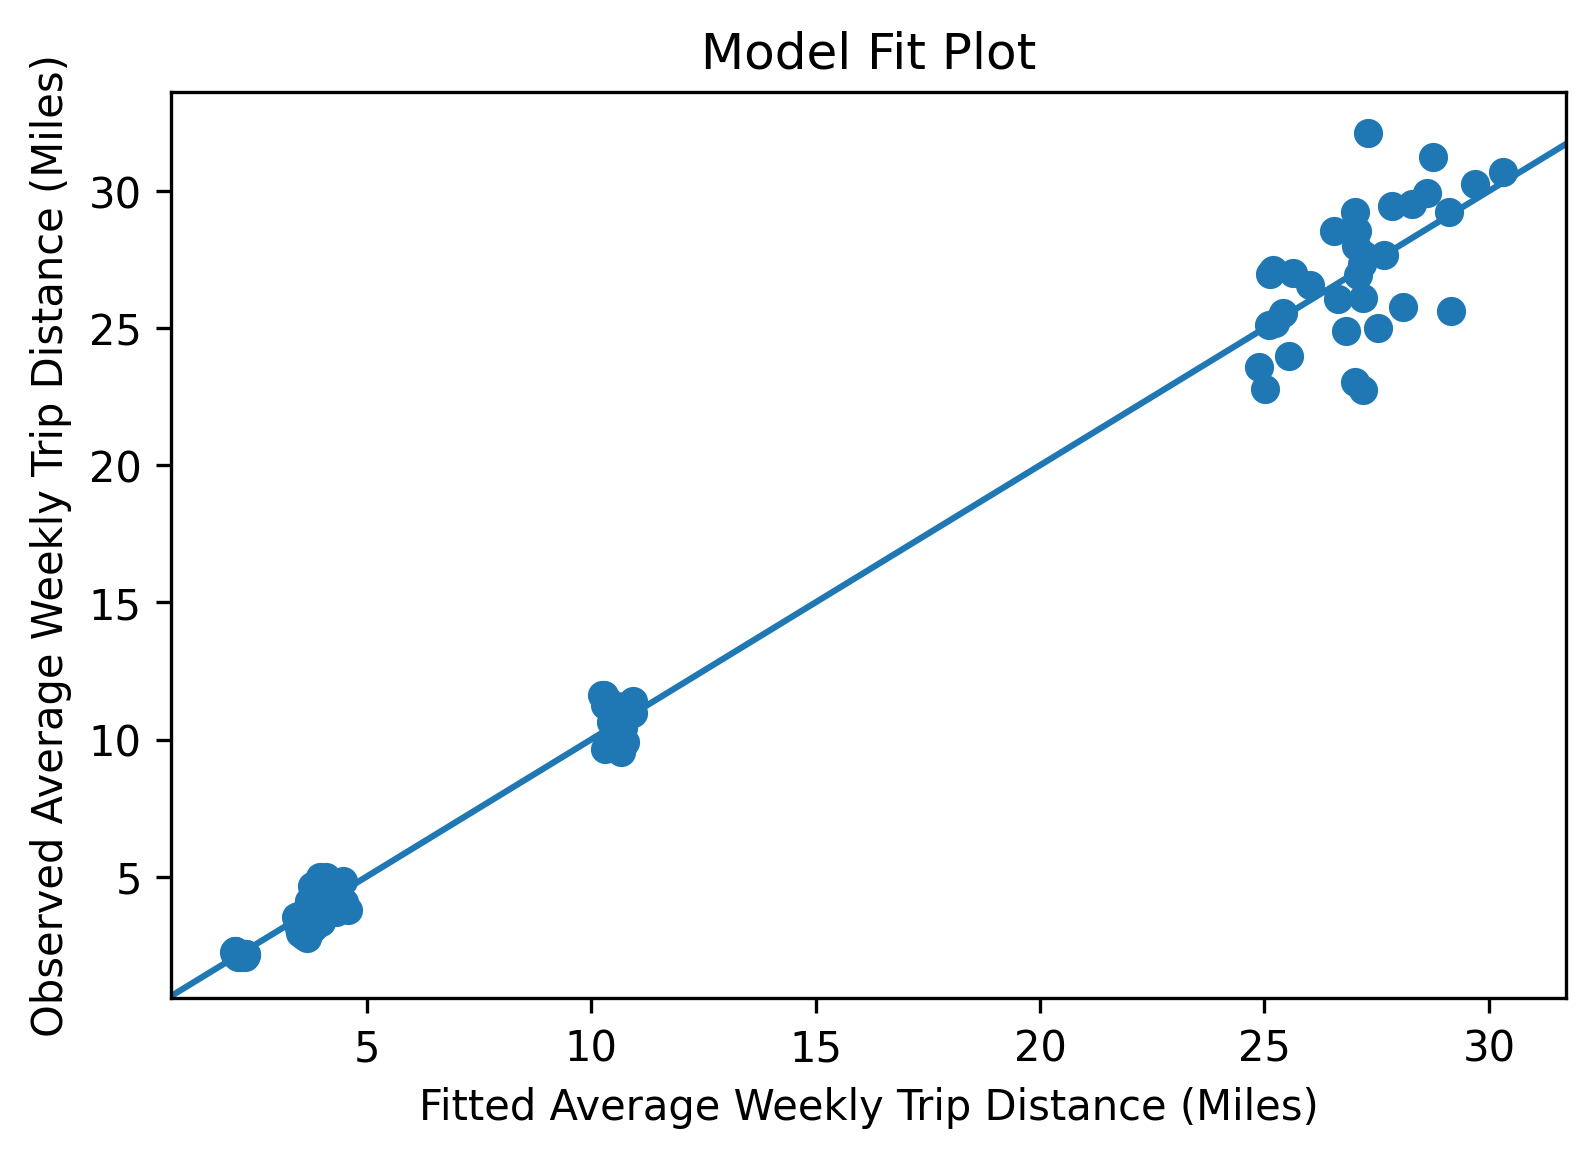
\includegraphics[width=0.51\textwidth]{../plots/diagnostic-Observed Average Weekly Trip Distance (Miles)-vs-Fitted Average Weekly Trip Distance (Miles).png}
        % this ensures your figures are centered where possible
        \centering
        \caption{How observed and fitted values compare for the trip distance OLS.} % refer to this image as (Figure 1)
        \label{fig:ols}
    \end{figure}

\end{multicols}

\begin{multicols}{2}
    \textbf{Weekly Average Passenger Count:}
The passenger count in each trip is a discrete metric
likely described by a Poisson distribution with a rate parameter $\lambda$, 
while the average passenger count/rate per trip per week is a rate value on a continuous scale.
If the data was aggregated per trip, then it could be modelled with a simple Poisson regression.
However, since the estimated rate of a Poisson random variable is complicated to model,
it is preferrable to model the total count of passengers in each trip in a week
using a Poisson regression with an offset equal to the logarithm of the number of trips \cite{poisson}.
This is derived using the log link function in a generalized linear model attempting to model passenger rate:

\begin{align*}
    \log \left[\frac{\text{Passenger Count}}{\text{Number of Trips}}\right] &= X\hat{\beta} \\
    \implies \log \left[\text{Passenger Count}\right] &= X\hat{\beta} \\
    &+ \log \left[\text{Number of Trips}\right]
\end{align*}

\end{multicols}
% \pagebreak
\begin{multicols}{2}

    \begin{figure}[H]
        % change the scale multiplier to make the figures smaller or larger
        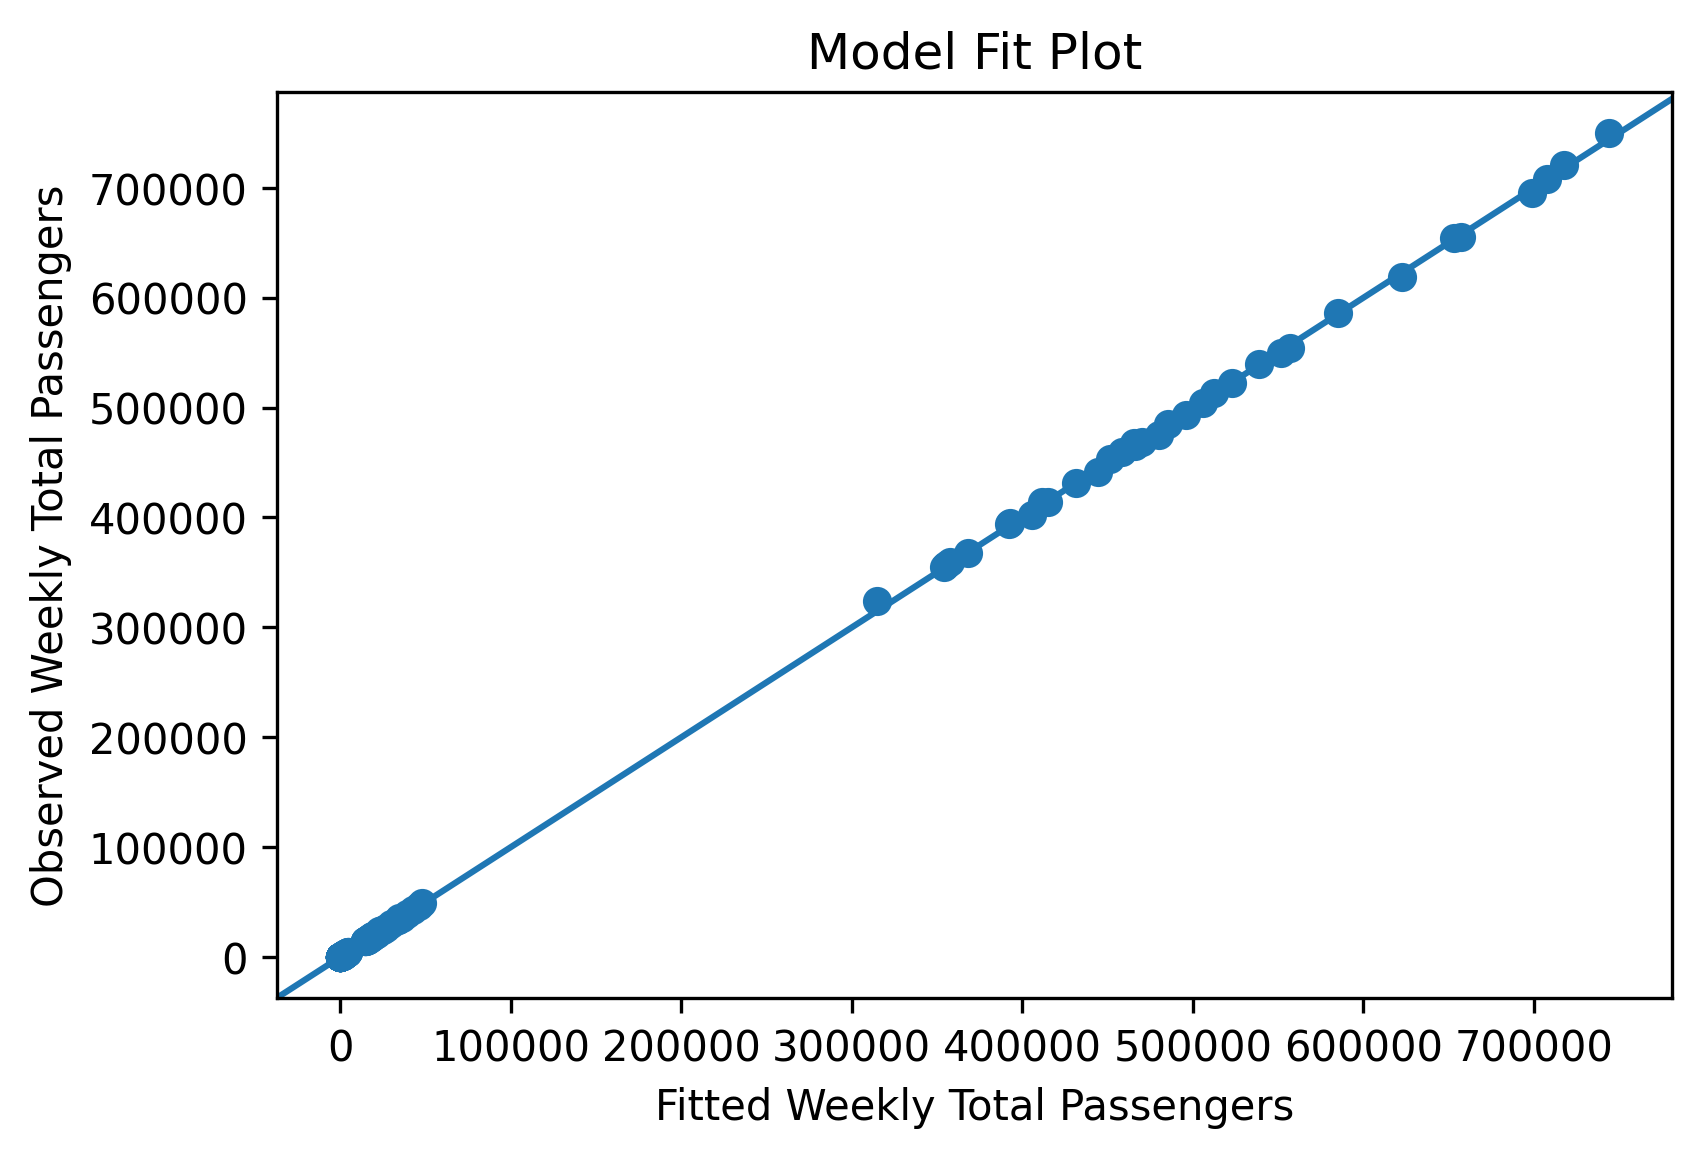
\includegraphics[width=0.51\textwidth]{../plots/diagnostic-Observed Weekly Total Passengers-vs-Fitted Weekly Total Passengers.png}
        % this ensures your figures are centered where possible
        \centering
        \caption{How observed and fitted values compare for total passenger counts in the Poisson regression.} % refer to this image as (Figure 1)
        \label{fig:glm}
    \end{figure}

    Again, there is no single solution for the parameters of this model due to the input data containing a categorical predictor.
Instead the resulting $p$-values for each parameters can be analyzed to see if any relationships are irrelevant to modelling passenger counts.
Specifically high is the $p$-value for the $z$ statistic of Influenza total cases with a value of $p = 0.415$, 
suggesting that with even a $95\%$ confidence level, 
Influenza has little correlation to reliance on taxis.
According to Figure~\ref{fig:glm}, this model appears to strictly conform to the observations given.
This might unfortunately also be an indicator of overfitting in the data,
which would require further data to be collected and checked against to confirm.

\end{multicols}



% \begin{enumerate} 
%     \item Example for enumerated points
%     % use \item to create more points
% \end{enumerate}

% \begin{itemize} 
%     \item Example for dot points
%     \item[*] You can change dot points to any symbols by putting [SYMBOL].
%     \item[$\times$] Here's a fun example.
% \end{itemize} 
% \lipsum[4-5]
% Example code for figures:
% % the [h] ensures your figure is inline at the location and not displayed on some other page
% \begin{figure}[h]
%     % change the scale multiplier to make the figures smaller or larger
%     \includegraphics[width=0.35\textwidth]{example-image-a}
%     % this ensures your figures are centered where possible
%     \centering
%     \caption{Some caption} % refer to this image as (Figure 1)
% \end{figure}
% \lipsum[1-2]

% Example of a maths equation:
% \begin{equation}
%     Y = X\beta + \epsilon
% \end{equation}

% Example of an aligned equation (\& denotes the symbol to align):
% \begin{align*}
%     E[\mathbf{y}] &= X\beta + E[0] \\
%                   &= X\beta
% \end{align*}

% Example of an in-line equation $\epsilon \sim N(0, 1)$ \\

\section{Conclusions}

This report provides a brief investigation into possible relationships between
incidences of viral infection within a certain borough, 
and the distances or passenger counts for taxi trips starting in that borough.
Since the generated linear models apply to different responses, 
they cannot be compared on how well they predict a common response, 
but on how strongly they display a relationship between the reliance measure
and viral case rates.
According to the linear models generated, the case rates of COVID-19 
are most relevant in predicting the following week's average trip distances 
and passenger counts. 
While the model for passenger counts appears to fit better than for trip distances,
this may be due to overfitting present in the underlying data.
On the trip distance model, using a linear regression may not result in the best
fit due to the presence of multimodal data.

It is important to note that no causal relationships were proven or investigated in this report,
and thus the generated models cannot be relied on as anything more than reflections
of underlying correlations. In the same vein, while the models can be used to predict future reliance measures of yellow taxis,
they should by no means be the only models relied upon, and should be used in conjunction several others.

To conclude, there appears to be a correlation between the case rates of COVID-19
and the distances and passenger counts of taxi trips in the following week.
Such a relationship is less strong with Influenza case rates. Therefore,
it cannot be concluded decisively if there is a common effect that increased disease 
in a persons vicinity will alter how they use common forms of transport.

\section{Recommendations}
This has been a thorough, but brief look into correlations between viruses and reliance metrics.
The following are several paths on which further research in this area could begin:
\begin{itemize}
    \item It should be considered that there are sevaral datasets which could be included
    in a similar analysis, such as considering other viruses, or considering other forms of transport.
    With more data to analyze, a clearer picture of the true relationships between infectious disease and preceived need for transport services.
    \item As mentioned in the paper, aggregation of TLC data performs grouping by pickup location.
    This means the same analysis should also be performed on aggregation by dropoff location instead.
    It would be interesting to compare and contrast the resulting models generated with this different grouping.
    \item Another way in which the research could be deepened would be to select a subset of specific locations where trips going to/from are likely work-related. 
    This would provide a window into measuring the shift to working from home caused by viruses.
\end{itemize}

\clearpage

% BEGIN REFERENCES SECTION
\printbibliography

\end{document}